\chapter{Deep Learning with Neural Nets}
	\label{cha:deep_learning}

	The nature of the research presented in this thesis is inter-disciplinary: machine intuition applied to cognitive network automation requires expertise in both deep learning, as well as in mobile networks.
	I have conducted my research at the Chair of Network Architectures and Services at the Technical University of Munich, and at Nokia (Bell-Labs).
	Thus, my research environment mostly consisted of networking experts, rather than data scientists or deep learning specialists.
	Understandably, my colleagues or my audience was often not versed in the specific deep learning algorithm at hand.
	Similarly, I also don't expect extensive deep learning experience from you, dear Reader of this thesis.
	
	I believe in the future this expectation will change, as deep learning will become an essential tool that is used in all technological fields.
	Future networking experts will have to utilize deep learning algorithms in their everyday work, similarly to the way we now use different programming languages, software or computational hardware like PCs or tablets regularly.
	For now, this chapter serves as an intensive course on deep learning components and techniques for networking experts who might have heard of some concepts, but never had to use or experiment with these algorithms in a hands-on fashion.
	
	This chapter summarizes \ac{DL} in a similar way to the following chapter in the \ac{CAN} book, which I co-authored:
	
	\begin{publication}
		Machine Learning: Tools for End‐to‐End Cognition \\
		\textit{Stephen S. Mwanje, Márton Kajó, Benedek Schultz} \\
		Towards Cognitive Autonomous Networks: Network Management Automation for 5G and Beyond (2020): 203-254.
	\end{publication}

	My contribution to the above book chapter was the authoring of the sections on deep learning, as well as general supervision, correction and editing of the whole chapter.
	The discussion in this thesis takes elements from the book, but expands on them with a more in-depth explanation of low-level concepts regarding neural nets, as well as high-level aspects of deep learning, altogether providing a more well-rounded introduction.
	This chapter also includes an overview of the use of \ac{DL} in mobile networks, as a way of providing a background on the state-of-the-art, but also to reinforce my previous statements on the problem of insufficient \ac{DL} research in our domain.
	
	Naturally, the information regarding deep neural nets is available in other publications in more detail.
	For an excellent in-depth read, I recommend \cite{deep_learning_book}.
	Please note, that any statement in this chapter that would otherwise require a reference, is taken from this recommended book.
	
	\section{Basic Neural Nets}
	
		\subsection{Fully-connected Layers}
	
			\emphix{Neural nets}{neural net} are directed computational graphs: edges transmit and scale values, while nodes accumulate and transform values through various functions.
			The basic building block of a neural net is a \emphix{neuron}{neuron}.
			Much like a human neuron, it incorporates a node (nucleus) and several connected edges (synapses), which transmit incoming values towards the node (Fig.~\ref{fig:neuron}).
			While transmitting values, the edges scale (weigh) the values according to learned parameters (weights).
			The accumulation is done through the summation of the incoming scaled values and an additive bias term, which is also learned.
			With all this combined, a neuron realizes the following simple function:
			\begin{equation}
				\label{eq:neuron}
				y = \sum_{j=1}^{n_i} x_{j}w_{j} + b,
			\end{equation}
			\noindent where $x_j$ denotes incoming values, $w_j$ scaling weights, $b$ the added bias and $y$ the output of the neuron.
			
			\begin{figure}[ht]
				\centering
				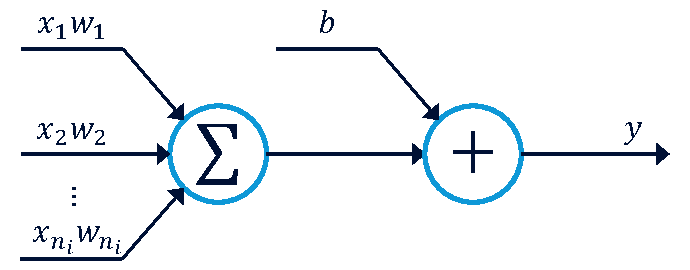
\includegraphics[width=0.46\linewidth]{figures/02_deep_learning/neuron/neuron.pdf}
				\caption[Neuron]{The basic building block of a neural net: a neuron.}
				\label{fig:neuron}
			\end{figure}
			
			Although neural nets allow for irregular graph topologies (and are in fact sometimes used this way), they are almost always used in a more structured topology.
			Most neural nets are \emphix{feedforward}{feedforward}: neurons are organized into \emphix{layers}{layer}, so that connections run between neurons in neighboring layers, but not between neurons in the same layer.
			Furthermore, connections always run from the ``earlier'' layer (the layer closer to the input) towards the ``later'' layer (the layer closer to the output of the net).
			One exception to this rule are recurrent nets: although mostly made up of feedforward subnets, there are \emphix{recurrent}{recurrent} connections, which feed backward into earlier parts of the net.
			Recurrent nets will be discussed later in more detail (Sec.~\ref{cha:deep_learning:sec:recurrent_nets}), but for now, we can concentrate on feedforward nets.
			Feedforward nets are often described as having an ``input'' and an ``output'' layer -- which act as interfaces to the outside of the neural net -- as well as a various amount of \emphix{hidden}{hidden layer} internal layers in-between.
			
			\begin{figure}[ht]
				\centering
				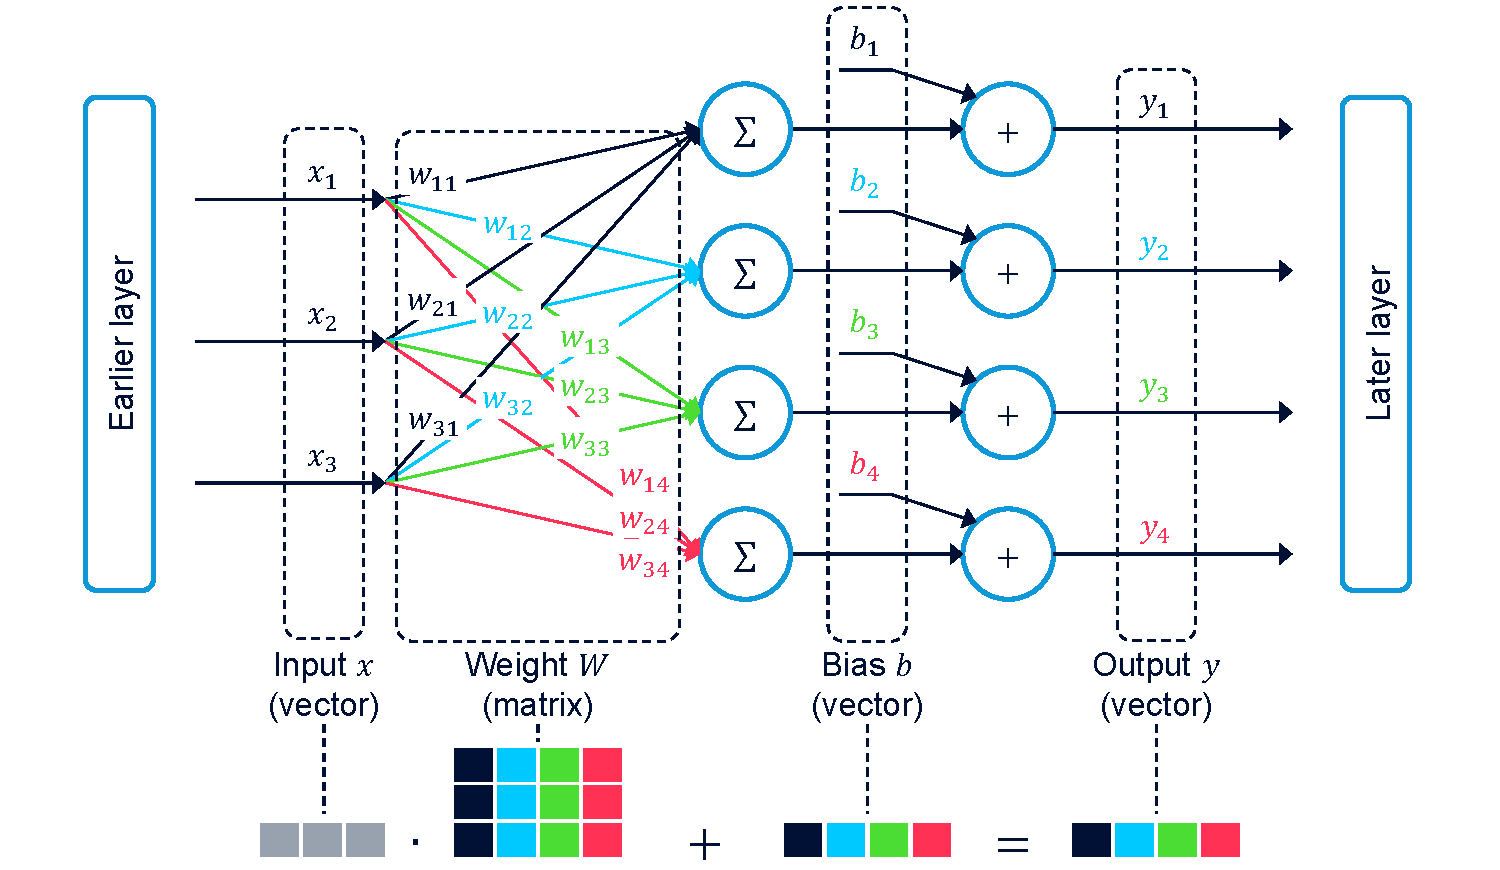
\includegraphics[width=\linewidth]{figures/02_deep_learning/fc_layer/fc_layer.pdf}
				\caption[Fully-connected layer]{An example of a fully-connected layer.}
				\label{fig:fc_layer}
			\end{figure}
			
			If we lay out the previously described neurons ``side-by-side'' to build a layer, and connect every neuron in the current layer to every neuron in the previous layer, we get what is called a \emphix{\ac{FC}}{fully-connected layer} layer.
			\ac{FC} layers are the earliest commonly used neural net building blocks, and can still be found in almost every state-of-the-art net topology.
			A notable exception to this are convolutional nets made up entirely of convolutional layers.
			However, convolutional layers can be derived from \ac{FC} layers, as we will see in Sec. \ref{cha:deep_learning:sec:convolutional_nets}.
			An example of a fully-connected layer can be seen in Fig.~\ref{fig:fc_layer}.
			Because of the fully-connected subgraph between the two layers, the weighted transmission through the connecting edges can be written in a simplified form, as a matrix-multiplication between the \emphix{input vector}{input vector} of the layer and its \emphix{weight matrix}{weight!matrix}.
			Furthermore, the additive bias can also be calculated as a vector addition, arriving at the vectorized form of a \ac{FC} layer:
			\begin{equation}
				\label{eq:fc_layer}
				\mathbf{y}_{(1 \times n_o)} = \mathbf{x}_{(1 \times n_i)}\mathbf{W}_{(n_i \times n_o)} + \mathbf{b}_{(1 \times n_o)},
			\end{equation}
			\noindent where $n_i$ represents the number of features in the input, $n_o$ the number of neurons in the current layer, $\mathbf{y}_{(1 \times n_o)}$ denotes the $n_o$-width horizontal output vector, $\mathbf{x}_{(1 \times n_i)}$ denotes the $n_i$-width horizontal input vector, $\mathbf{W}_{(n_i \times n_o)}$ the $n_i \times n_o$ sized weight matrix, $\mathbf{b}_{(1 \times n_o)}$ the $n_o$-width horizontal bias vector.
			This vectorized calculation is also exemplified on the bottom of Fig.~\ref{fig:fc_layer}.
			At this point, I would urge the Reader to stop thinking about neural nets as computational graphs.
			What is realized in neural nets are essentially a sequence of matrix multiplications, element-wise additions and element-wise functional transformations.
			I think it is better to imagine each neural net as a sequence of linear-algebraic or even geometrical functions, a mental image that I will extensively use in explanations throughout this dissertation.
		
			In this currently discussed state, \ac{FC} layers are quite limited in their modeling capability.
			The geometric function that is realized through a \ac{FC} layer is an \emphix{affine mapping}{affine mapping}: a composition of a linear mapping (projection by multiplication through $\mathbf{W}$) and a translation of the input vector (addition of $\mathbf{b}$).
			For our discussion, an important property of affine maps is that a chain of multiple affine maps can always be simplified into a single affine map \cite{linalg_book}.
			Thus, even if the net consists of multiple \ac{FC} layers, the realizable function can be still collapsed into a singular \ac{FC} layer.
			This effectively limits the modeling capability of a neural net purely made of \acp{FC} layers to \emphix{linear regression}{linear regression}.
			Correspondingly, \ac{FC} layers are also often called linear layers because of this.
			To escape this limitation, a critical component needs to be introduced to the net: nonlinearities.
		
		\subsection{Generic Function Approximation with Step Nonlinearity}
		
			% Vertical alignment: https://tex.stackexchange.com/questions/378548/vertical-alignment-of-side-by-side-minipages
			\begin{figure}[ht]
				\centering
				\begin{minipage}[t]{0.4\linewidth}
					\begin{equation}
						y = \begin{cases}
						0 & if\; \sum_{j=1}^{m} x_{j}w_{j} < b, \\
						1 & if\; \sum_{j=1}^{m} x_{j}w_{j} > b,
						\end{cases}
					\end{equation}
				\end{minipage}
				\begin{minipage}[t]{0.3\linewidth}
					\raisebox{-0.85\height}{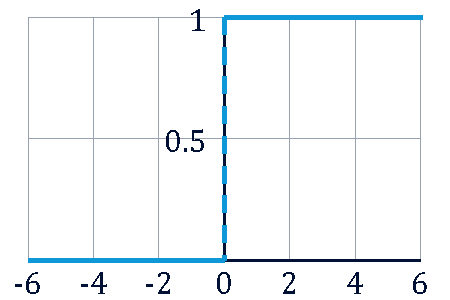
\includegraphics[width=\linewidth]{figures/02_deep_learning/nonlins/step.pdf}}
				\end{minipage}
				\caption[Step nonlinearity]{The gate-like effect of the step nonlinearity.}
				\label{fig:nonlins_step}	
			\end{figure}
			
			Early researchers envisioned neural nets as programmable logical circuits \cite{neocognitron}.
			To implement logic, in this early iteration neurons were meant to resemble logical AND or NAND gates, the idea being that NAND gates are universal for computation, and that any logic circuit can be built using them.
			In order to realize this, the hard step-function was used to limit the output of a neuron to the binary $0$ or $1$.	
			In this setup, the neuron-gate flips depending on the weighted sum of the inputs, with the bias acting as the decision threshold for the flip (Fig.~\ref{fig:nonlins_step}).
			The step function can be seen as the first nonlinearity that was utilized in neural nets.
			A \ac{FC} neuron combined with the step nonlinearity in early neural nets was called a perceptron, and neural nets built using these were called as \acp{MLP}, a term still in use to refer to neural nets using \ac{FC} layers.
			I would like to note here that the literature often refers to this combination of a \ac{FC} layer and a nonlinearity together as a ``layer'', and discusses the combined aspects as a singular entity.
			This logic is further supported by the fact that \ac{FC} layers are almost always followed by nonlinearities, thus discussing them as one element made practical sense.
			However, in my opinion, it is much more flexible to refer to nonlinearities as their own layers, and I will use this nomenclature hereafter.
			
			The addition of even this basic nonlinearity elevates the modeling capability of a neural net to one of a \emphix{generic function approximator}{generic function approximator}: a model that is capable of approximating any continuous mathematical function, to a certain accuracy.
			To illustrate this property, we can use a simple neural net comprised of a \ac{FC} layer of $m$ neurons, followed by the step-function nonlinearity, and ending in a \ac{FC} layer of a single neuron.
			This simple neural net is capable of approximating any desired $f(x) = y$ through a series of steps: each neuron in the first \ac{FC} layer acts as the before mentioned gate, creating a step at learned biases $b_j$ (Fig.~\ref{fig:generic_approximator}).
			The weights of the second \ac{FC} layer set the sizes of the steps.
			Already an interesting observation here is that for pure \emphix{regression}{regression} tasks (i.e.: approximating a continuous mathematical function), it is not beneficial to have a nonlinearity after the last \ac{FC} layer, rather, nonlinearities are only present after internal (hidden) layers.
			
			\begin{figure}[ht]
				\centering
				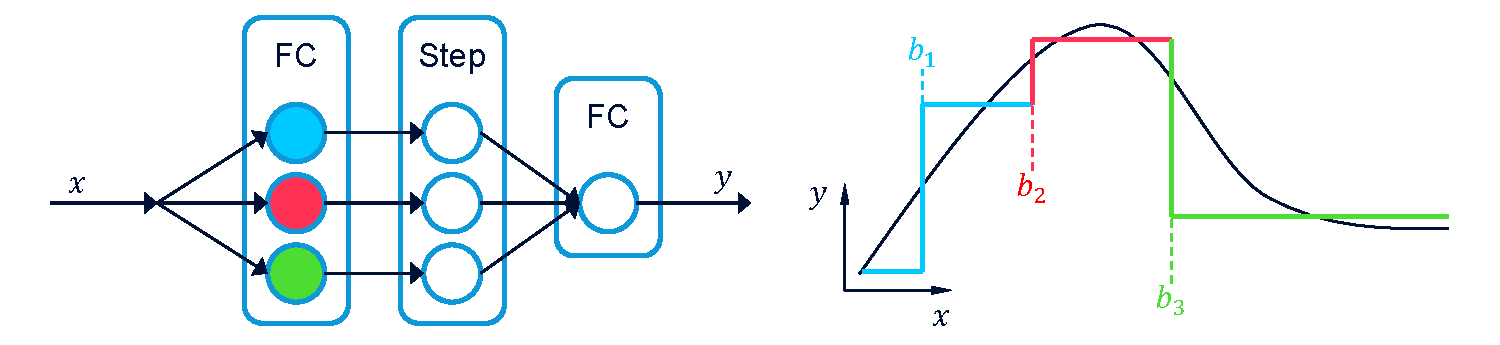
\includegraphics[width=\linewidth]{figures/02_deep_learning/generic_approximator/generic_approximator.pdf}
				\caption[Generic function approximation with MLPs]{Illustration of the generic function approximator capability of FC layers combined with a step nonlinearity.}
				\label{fig:generic_approximator}
			\end{figure}
			
			A series of these steps can approximate a function to a certain degree, limited by the number of steps available.
			In order to be able to achieve a better approximation, the first \ac{FC} layer would need to be \emphix{wider}{layer!width}, i.e.: contain more neurons.
			It is easy to see that theoretically, an infinitely wide first \ac{FC} layer could perfectly approximate any function, even if the input or output is not $1$-dimensional \cite{neuralnetsanddeeplearning}.
			However, the topic of this dissertation is not wide learning, but deep learning.
			\emphix{Deep}{neural net!depth} refers to the depth of the neural nets, i.e.: how many layers make up the net.
			The more layers a net contains, the deeper it is.
			But if any function can be theoretically approximated by a wide-enough single-hidden-layer net, why would we need to stack multiple layers on top of each other?
			
			We can imagine a single layer as a model capable of formulating rules, or learning filters upon which its specific neurons are triggered.
			If the output of a previous layer is processed by a subsequent layer, the net essentially formulates rules upon rules, e.g.: models a set of \emphix{hierarchical rules}{hierarchical rules} \cite{neuralnetsanddeeplearning}.
			A wide net is capable of learning many simple rules in parallel, whereas a deep net is capable of learning complex hierarchical rules.
			Hierarchical rules are closer to how human reasoning works, and thus are more fitting to the real-world cognitive tasks neural nets are utilized for.
			A good example of this is human vision: our brain detects atomic geometrical forms first (edges), which are then combined into more complex shapes, which are then further related to each other to detect complete objects in our vision.
			The learned rules are often referred to as \emphix{filters}{filter} or \emphix{features}{feature}.
			The hierarchical features learned by deep neural nets will be further explored in Sec.~\ref{cha:deep_learning:sec:hierarchical_features}.
			Furthermore, although many processing tasks could be approximated by single wide layers, they can often be realized by fewer components -- parameters in this case -- if they are organized into multiple layers.
			Thus, the effective modeling power of deeper nets is relatively larger than their wide counterparts, using the same amount of parameters. 
	
		\subsection{Logistic Nonlinearities, Regression and Classification}
		
			As early neural nets utilizing perceptron-neurons were either not learning machines (using preset weights), or trained through global optimization (such as genetic algorithms), the non-continuous nature of the step function wasn't a problem.
			However, as soon as neural nets were being trained through means of derivative optimization, a continuous activation function was needed.
			The earliest approach was to use a nonlinear continuous function that is quite similar to the step function.
			The group of functions used for this purpose are the \emphix{sigmoid}{sigmoid} functions, the most prominent being the logistic function (which is often called \emphnox{the} sigmoid function), and its shifted and scaled variant to the $[-1, 1]$ interval, the tangent-hyperbolic function.
			
			\begin{figure}[ht]
				\centering
				\begin{minipage}[t]{0.4\linewidth}
					\begin{equation}
						\sigma(x) = \frac{1}{1+e^{-xk}}
					\end{equation}
				\end{minipage}
				\begin{minipage}[t]{0.3\linewidth}
					\raisebox{-0.7\height}{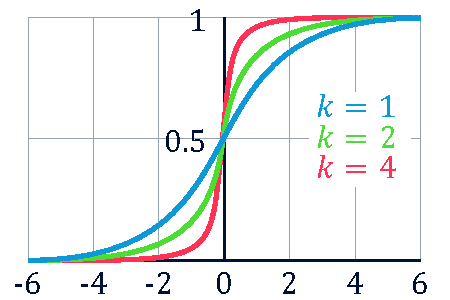
\includegraphics[width=\linewidth]{figures/02_deep_learning/nonlins/sigmoid.pdf}}
				\end{minipage}
				\caption[Sigmoid nonlinearities]{Sigmoid (logistic) nonlinearities.}
				\label{fig:nonlins_sigmoid}
			\end{figure}
		
			The logistic sigmoid nonlinearity can be seen in Fig.~\ref{fig:nonlins_sigmoid}.
			The logistic growth rate $k$ changes the shape of the function, which looks more and more similar to a step function as $k$ increases.
			It is easy to imagine that using a high $k$ value is preferable to reproduce the hard-decision-like behavior of the step function, and retain a close similarity to perceptrons.
			However, a high $k$ value is not necessary to emulate a steeper decision boundary: as the sigmoid is preceded by a \ac{FC} layer, it is enough to learn high weights on the inputs to achieve a quick flip around the bias.
			Thus, although $k$ makes it easier to see why sigmoid nonlinearities succeeded the step function, the $k$ parameter can be left out from the implementation without any downsides.
			Leaving out $k$ from the calculation also speeds up processing by skipping one extra multiplication.
			
			We have already talked about \nomphix{regression}{regression} as a task in the generic function approximation context.
			Literature on deep learning often organizes neural nets into different categories based on the tasks they undertake: regression, classification, transcription, structuring, translation, synthesis, imputation, denoising, etc..
			In my opinion, this categorization is a little meaningless: neural nets are function approximators, and in every task what they truly realize is regression.
			The overall task mostly changes the way the output is interpreted, but not the actual goal of regressing a desired (continuous) function.
			Often, the task-specific output interpretation is not even used for training, only in inference as a post-processing step.
			
			With that said, if possible, it certainly helps if a specific output-processing step can be implemented as a hard-coded function, instead of the neural net having to learn to output data in a specific way.
			The most important instance of this is \emphix{classification}{classification}: in this task, the neural net has to specify which of $k$ categories the input observations belong to.
			In order to do so, the output of the net has to resemble class-association probabilities: a $k$-long vector of values restricted to the $[0, 1]$ interval, where $0$ represents no chance of the input belonging to the class, while $1$ represents a guarantee that the input belongs to that class.
			Furthermore, the class-association vector values also have to sum to $1$ to resemble a probability distribution.
			To learn to output a vector that follows these restrictions is quite complicated in itself, not to mention actually guessing the correct class for every input.	
			In order to relieve the neural net from learning how to output class-association probabilities, usually a specific nonlinearity is used: the \emphix{softmax}{softmax layer} function.
			The softmax nonlinearity can be seen in Fig.~\ref{fig:nonlins_softmax}.
			Contrary to what we observed previously about nonlinearities only placed after hidden layers, the softmax nonlinearity is always placed as the last layer, and could be seen as a post-processing function.
			Through the division by the sum of the individual vector values, the softmax function ensures both that the output values fall within the $[0, 1]$ interval and that they sum to $1$.
			Furthermore, an interesting aspect of the softmax is that it has intra-layer dependency: the values in the same layer influence each other, if one value becomes larger, this will make all other values in the same output vector become smaller.
			
			\begin{figure}[ht]
				\centering
				\begin{minipage}[t]{0.4\linewidth}
					\begin{equation}
						\label{eq:sm}
						f_{SM}(x_j) = \frac{e^{x_j}}{\sum_{y=1}^{k} e^{x_y}}
					\end{equation}
				\end{minipage}
				\begin{minipage}[t]{0.3\linewidth}
					\raisebox{-0.7\height}{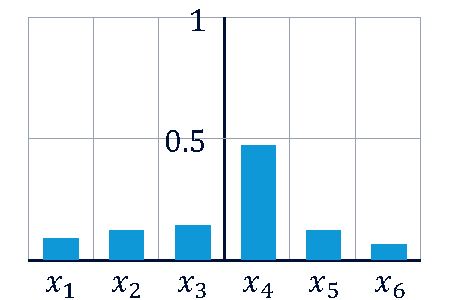
\includegraphics[width=\linewidth]{figures/02_deep_learning/nonlins/softmax.pdf}}
				\end{minipage}
				\caption[Softmax nonlinearity]{Softmax nonlinearity.}
				\label{fig:nonlins_softmax}
			\end{figure}
			
	\section{Neural Net Training}
	
		\subsection{Gradient Descent and Backpropagation}
			\label{cha:deep_learning:sec:sgd_backprop}
			
			The previous section discussed matrix multiplication and addition-based \ac{FC} layers, and element-wise sigmoid and softmax nonlinearities.
			These building blocks allow for the construction of ``basic'' neural nets, which made up the state-of-the-art for a long time, before the deep learning boom.
			These neural nets are often called \acp{FNN}, \acp{MLP} or incorrectly as the umbrella term \ac{ANN}.
			One crucial part of neural nets was only mentioned so far: learning.
			Neural nets are powerful because they are learning machines, and can extract rules and features from example observations.
			As we will see here, machine learning and neural nets are a perfect match: the simple atomic operations and the sequential nature of the nets allow for the efficient calculation of gradients, making gradient-based optimization the most prominent training method of neural nets and the enabler of today's deep learning.
	
			Modern neural nets learn through \emphix{gradient descent}{gradient!descent}.
			In this mathematical optimization paradigm, the task is to minimize a function $f(\mathbf{x})$ by changing its input $\mathbf{x}$.
			As I argued before, neural nets are function approximators, and because of this, naturally their own processing can also be seen as a function.
			Neural nets realize the function $\mathbf{y} = f_n(\mathbf{x}, \mathbf{\theta})$, where $x$ refers to the input, $\mathbf{\theta}$ represents all the learnable parameters in the net, and $\mathbf{y}$ is the output.	
			In supervised learning tasks, the goal is to minimize the difference between the actual output and a target output.
			In unsupervised learning, this goal is usually a little more complicated, either having additional constraints on the output or not having a target output at all.
			For the illustration of gradient descent in this section, I will stick to discussing the simpler supervised learning task.
				
			In order to realize the minimization of the difference between actual and target output through gradient descent, a singular value is needed to represent this difference, called \emphix{loss}{loss} ($l$).
			To arrive at the loss value, neural nets require a \emphix{loss function}{loss!function} ($f_l(\mathbf{y}, \mathbf{y}')$), which is used to calculate this difference between the actual ($\mathbf{y}$) and the target ($\mathbf{y}'$) output.
			Loss functions are also commonly referred to as objective functions, cost functions or error functions, but	I will try to use the term loss function consistently in this dissertation.		
			For the most part, loss functions measure the difference between the actual and target output of the net.
			Gradient descent training is usually highly sensitive to the type of loss function used, thus it is critical to choose the correct loss function for the given task.
			The two most commonly used loss functions are:
			\begin{itemize}
				\item \textbf{\ac{MSE}} is usually utilized for regression tasks. The \ac{MSE} loss measures the squared Euclidean distance between vectors $y_{(1 \times d)}$ and $y'_{(1 \times d)}$ containing  $d$ dimensions:
				\begin{equation}
				l_{MSE} = \frac{1}{d} \sum_{j=1}^{d} (y'_{j} - y_{j})^2
				\end{equation}		
				
				\item \textbf{\ac{NLL}} is usually utilized for classification tasks. \ac{NLL} estimates the likelihood of two vectors $y_{(1 \times d)}$ and $y'_{(1 \times d)}$ containing a probability distribution for $d$ classes:
				\begin{equation}
				\label{eq:nll}
				l_{NLL} = -\sum_{j=1}^{d} y'_{j}\ln{y_{j}}
				\end{equation}
			\end{itemize}
			
			\noindent While \ac{MSE} is capable of measuring the distance between any two vectors, \ac{NLL} is only well-suited for values limited to the $[0,1]$ range.
			Furthermore, \ac{NLL} usually uses hard targets, where the $y'$ vectors have only a single value which is $1$, while the rest is $0$.
			These vectors are often called \emphix{one-hot vectors}{one-hot vector}: the position of the $1$ in the vector encodes the correct class label/index.
			One-hot encoded $y'$ vectors also simplify the $l_{NLL}$ calculation, as only one of the components will be non-zero.
			Because the \ac{NLL} is used in classification tasks, it is almost always preceded by a softmax nonlinearity.
			Fortunately, there is a great synergy between the softmax nonlinearity and the \ac{NLL} loss, and produce a very simple gradient formula when used together.		
			
			Using the loss functions, we can write the gradient descent optimization goal for neural nets as:
			\begin{equation}
				\label{eq:gradient_descent_loss}
				l = f_l(f_n(\mathbf{x}, \mathbf{\theta}), \mathbf{y}'),
			\end{equation}
			\begin{equation}
				\label{eq:gradient_descent_goal}
				l^* = arg\:\underset{\theta}{min}\:f_l(f_n(\mathbf{x}, \mathbf{\theta}), \mathbf{y}'),
			\end{equation}
			\noindent where $l^*$ refers to the minimal loss value measured on $y = f_n(\mathbf{x}, \mathbf{\theta})$ and $\mathbf{y}'$, achieved by optimizing the learnable net parameters $\mathbf{\theta}$.
			
			\begin{figure}[ht]
				\centering
				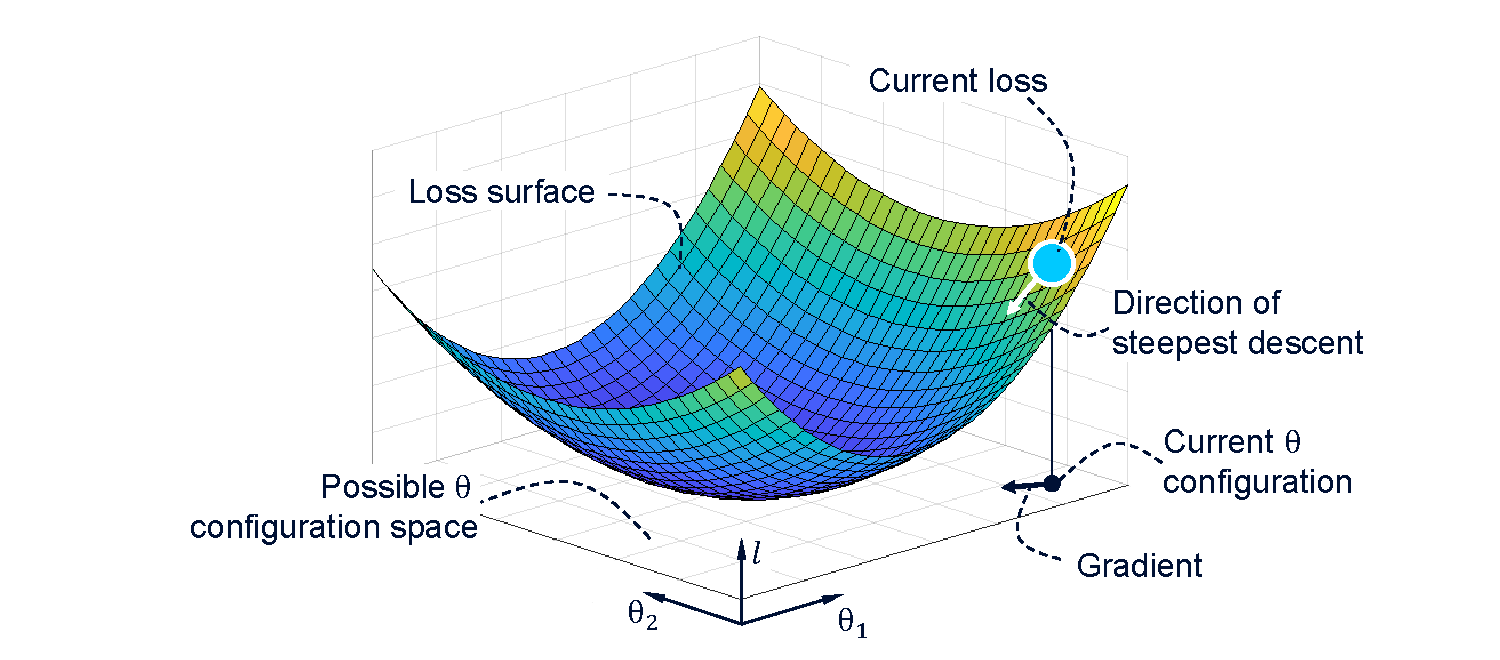
\includegraphics[width=\linewidth]{figures/02_deep_learning/gradient_descent/gradient_descent.pdf}
				\caption[Gradient descent illustration]{Illustration of gradient descent.}
				\label{fig:gradient_descent}
			\end{figure}
			
			Gradient descent is best imagined as a search for the lowest point, where the loss values at different $\mathbf{\theta}$ configurations create a topological ``surface'' (as illustrated in Fig.~\ref{fig:gradient_descent}).
			The possible $\mathbf{\theta}$ configurations can also be seen as a space, where a single point sets all neural net parameters to a certain value.
			The goal is then to move in the $\mathbf{\theta}$ space to a position, which corresponds to the lowest point on the loss surface.
			Because neural nets realize complex nonlinear functions and work on datasets which produce complex (non-convex) loss surfaces, generally finding the point in the $\mathbf{\theta}$ space which minimizes the loss cannot be solved in a closed form or by exhaustive search.
			Instead, gradient descent is an iterative and locally greedy search algorithm:
			\begin{itemize}
				\item \textbf{Iterative:} At every iteration, the loss is recalculated using training examples $\mathbf{x}$ and the corresponding output targets $\mathbf{y}'$, and the $\mathbf{\theta}$ parameters are changed to lower the loss.
				The change in $\mathbf{\theta}$ is restricted to be small, because it is generally unknown what the loss is going to be at the next iteration point (before actually calculating it), it is only assumed that small changes in $\mathbf{\theta}$ result in small and predictable changes in $l$.
				This creates a tradeoff between training accuracy and speed: larger steps at every iteration might lower the overall number of required iterations, speeding up training, at the expense of worse precision in the $\mathbf{\theta}$ point placement, and the higher potential of the training getting lost far from the global optimum.
				% Solution is per-parameter adaptive learning rates
				
				\item \textbf{Greedy:} Gradient descent is greedy, because at every iteration, $\mathbf{\theta}$ is changed in a way which has the most impact (largest decrease) in the loss value locally.
				Because of this local greediness, there is no guarantee that gradient descent finds a global optimum, as it is possible that the optimization gets stuck in saddle points or local minima on the loss surface.
			\end{itemize}
		
			I will discuss optimization schemes which mitigate many of the downsides stemming from the above two aspects in Sec.~ \ref{cha:deep_learning:sec:gradient_stab}.
			For now, the biggest question is how to determine the locally best direction in $\mathbf{\theta}$ which most effectively lowers the loss: the direction of steepest descent.
			Because $\mathbf{\theta}$ usually contains more than one parameter (i.e.: it is a vector), Eq.~\ref{eq:gradient_descent_loss} is a function with multiple inputs.
			If we want to know how the loss $l$ changes with regards to a single $\theta_i$ parameter, we can calculate the \emphix{partial derivative}{partial derivative} of the loss value:
			\begin{equation}
				\frac{\delta{l}}{\delta\theta_i} = \frac{\delta{f_l(f_n(\mathbf{x}, \mathbf{\theta}), y')}}{\delta\theta_i}.
			\end{equation}
			\noindent Calculating all the partial derivatives of the $\theta$ vector and organizing these also into a vector gives us the \emphix{gradient}{gradient}:
			\begin{equation}
				\nabla_{\theta}l = (\frac{\delta{l}}{\delta\theta_1}, \frac{\delta{l}}{\delta\theta_2}, ..., \frac{\delta{l}}{\delta\theta_i}).	
			\end{equation}
			\noindent The gradient can be seen as a vector pointing in the direction of steepest ascent in the $\theta$ space.
			It is logical that the steepest descent is in the exact opposite direction.
			In order to descend on the loss surface in the steepest direction, we can update the $\theta$ parameters in the following way ($\leftarrow$ refers to assignment):
			\begin{equation}
				\label{eq:gradient_descent}
				\mathbf{\theta} \leftarrow \mathbf{\theta} - \epsilon\nabla_{\theta}l,
			\end{equation}
			\noindent where $\epsilon$ is a small, positive scalar known as the \emphix{learning rate}{learning rate}, which is meant to restrict the updates to small changes, as previously mentioned.
			
			Applying the rule in Eq.~\ref{eq:gradient_descent} repeatedly will descend on the loss surfaces until reaching a minimum point, but to do this the gradient has to be also repeatedly calculated for multiple training points.
			This process could be quite computationally intensive, so for the effective training of neural nets, a simple and computationally inexpensive procedure is needed; fortunately, this is where the synergy between neural nets and gradient descent comes into play, because neural nets have a very effective way of calculating the gradient with regards to the loss.
			Every neural net layer can be seen as a function applied on the previous layer's output.
			As an example, let us discuss a neural net containing $2$ layers realizing the $2$ functions $y_1 = f_1(\theta_1, x)$ and $y_2 = f_2(\theta_2, y_1)$, and a loss function $l = f_l(y', y_2)$.
			The sequential nature of layers allows us to define the complete processing of this net as a chain (a composite) of functions:
			\begin{equation}
				l = f_l(y', f_2(\theta_2, f_1(\theta_1, x))).
			\end{equation}
			\noindent According to the chain rule, composite function derivatives can be calculated as:
			\begin{equation}
				\frac{\delta}{\delta{x}}z(y(x)) = \frac{\delta{z}}{\delta{y}}\frac{\delta{y}}{\delta{x}}.
			\end{equation}
			\noindent Using the chain rule, we can compute the partial derivative of the loss with regards to the parameters in the first layer as:
			\begin{equation}
				\label{eq:derivative_chain}
				\frac{\delta{l}}{\delta\theta_1} = \frac{\delta{f_l(y', y_2)}}{\delta{y_2}}\frac{\delta{f_2(\theta_2, y_1)}}{\delta{y_1}}\frac{\delta{f_1(\theta_1, x)}}{\delta{\theta_1}}.
			\end{equation}
			
			Equation~\ref{eq:derivative_chain} highlights an important aspect: in order to obtain partial derivatives, we can compute the derivatives of layers using only their own inputs and outputs.
			This suggests an implementation where layer outputs can be sequentially calculated once and stored (forward propagation), so that when calculating the partial derivatives backward in the sequence, these intermediate outputs can be reused without additional computation (backward propagation).
			This idea is the core of \emphix{backpropagation}{backpropagation}: the technique with which neural nets compute the partial derivatives of the loss with regards to every trainable parameter in the net.
			The name stems from the sequential forward- and backward calculations: the loss is effectively ``backpropagated'' through the net.
			The partial derivatives form the gradient, which is then used in the gradient descent optimization to update the trainable parameters of the net.
			To calculate the gradient, it is enough to have the derivatives of each layer defined in order to be able to implement the backpropagation algorithm.
			\ac{FC} layers have derivatives which can be calculated through simple matrix multiplication, while all other nonlinearities or losses have simple, predefined derivatives, also often calculated using stored intermediate outputs.
			The complete gradient descent algorithm can be seen on Alg. \ref{alg:gradient_descent}.
			
			\begin{algorithm}[!ht]
				\SetAlgoLined
				\newcommand{\nosemic}{\SetEndCharOfAlgoLine{\relax}}   % Drop semi-colon
				\newcommand{\dosemic}{\SetEndCharOfAlgoLine{\string;}} % Reinstate semi-colon
				\newcommand{\pushline}{\Indp}                          % Indent
				\newcommand{\popline}{\Indm\dosemic}                   % Undent		
				\let\oldnl\nl                                          % Store \nl in \oldnl
				\newcommand{\nonl}{\renewcommand{\nl}{\let\nl\oldnl}}  % Remove line number for one line
		
				\SetKwProg{forward}{Propagate Forward}{}{}
				\SetKwProg{loss}{Calculate Loss}{}{}
				\SetKwProg{backward}{Propagate Backward}{}{}
				\SetKwProg{update}{Update Parameters}{}{}
				
				\SetKwInput{Kw}{Required}
				\Kw{Neural net of $l$ layers: \ac{FC} layers and $f_{sigm}()$ sigmoid nonlinearities}
				\Kw{$f_l()$ loss function}
				\Kw{Learnable parameters: $\mathbf{W}_i, i\in\{1, ..., l\}$ weight matrices and $\mathbf{b}_i, i\in\{1, ..., l\}$ bias vectors}
				\Kw{Training dataset: $\mathbf{x}$ input vector and $\mathbf{y}'$ target output vector}
				\Kw{Learning rate $\epsilon$}
				
				\nosemic\nonl \;
				
				\dosemic\nonl\forward{}{
					\nosemic\nonl Calculate and store intermediate layer outputs: \;
					\dosemic $\mathbf{y}_0 = \mathbf{x}$\;
					\For{$i = 1, 2, ..., l-1, l$}{
						\uIf{\ac{FC} layer}{
							$\mathbf{y}_i \leftarrow \mathbf{y}_{i-1}\cdot\mathbf{W}_i + \mathbf{b}_i$\;
						}
			  			\uElseIf{Sigmoid nonlin.}{
							$\mathbf{y}_i \leftarrow f_{sigm}(\mathbf{y}_{i-1})$\;
						}
					}
					$\mathbf{y} = \mathbf{y}_l$\;
				}
				\nonl\loss{}{
					$l = f_l(\mathbf{y}', \mathbf{y})$\;
				}
				\nonl\backward{}{
					\nosemic\nonl Propagate the gradient to the output layer (behind the loss): \;
					\dosemic $\mathbf{g} \leftarrow \nabla_y{l} = \nabla_y{f_l(\mathbf{y}', \mathbf{y})}$\;			
					\For{$i = l, l-1, ..., 2, 1$}{
						\uIf{Sigmoid nonlin.}{
							\nosemic\nonl Propagate the gradient behind the nonlinearity: \;
							\dosemic $\mathbf{g} \leftarrow \nabla_{y_{i-1}}{l} = \mathbf{g} \circ f'_{sigm}(\mathbf{y}_{i-1})$\;
						}
						\uElseIf{\ac{FC} layer}{
							\nosemic\nonl Calculate the gradient on weights and biases: \;
							\dosemic $\nabla_{b_i}{l} \leftarrow \mathbf{g}$\;
							$\nabla_{W_i}{l} \leftarrow \mathbf{g} \cdot \mathbf{y}^T_{i-1}$\;
							\nosemic\nonl Propagate the gradient to the previous layer: \;
							\dosemic $\mathbf{g} \leftarrow \nabla_{y_{i-1}}{l} = \mathbf{g} \cdot \mathbf{W}^T_{i} $\;
						}
					}
				}	
				\nonl\update{}{
					\For{$i = 1, 2, ..., l-1, l$}{
						\uIf{\ac{FC} layer}{
							$\mathbf{b}_i \leftarrow \mathbf{b}_i - \epsilon\nabla_{b_i}{l}$\;
							$\mathbf{W}_i \leftarrow \mathbf{W}_i - \epsilon\nabla_{W_i}{l}$\;
						}
					}
				}
			
				\caption[Gradient descent]{A single iteration of \emphix{gradient descent}{gradient!descent} in a simple neural net. The ($\cdot$) operator refers to matrix-multiplication, while the ($\circ$) refers to element-wise multiplication (Hadamard product).}
				\label{alg:gradient_descent}
			\end{algorithm}
		
	%	\subsection{Backpropagation of Losses}
	%
	%		I have not yet discussed a critical component of the training of neural nets: loss functions.
	%		For the most part, loss functions measure the difference between the actual and target output of the net.
	%		Gradient descent training is usually highly sensitive to the type of loss function used, thus it is critical to choose the correct loss function for the given task.
	%		The two most commonly used loss functions are:
	%		\begin{itemize}
	%			\item \textbf{\ac{MSE}} is usually utilized for regression tasks. The \ac{MSE} loss measures the squared Euclidean distance between vectors $y_{(1 \times d)}$ and $y'_{(1 \times d)}$ containing  $d$ dimensions:
	%			\begin{equation}
	%				l_{MSE} = \frac{1}{d} \sum_{j=1}^{d} (y'_{j} - y_{j})^2
	%			\end{equation}		
	%	
	%			\item \textbf{\ac{NLL}} is usually utilized for classification tasks. \ac{NLL} estimates the likelihood of two vectors $y_{(1 \times d)}$ and $y'_{(1 \times d)}$ containing a probability distribution for $d$ classes:
	%			\begin{equation}
	%				\label{eq:nll}
	%				l_{NLL} = -\sum_{j=1}^{d} y'_{j}\ln{y_{j}}
	%			\end{equation}
	%		\end{itemize}
	%	    
	%		\noindent While \ac{MSE} is capable of measuring distance between any two vectors, \ac{NLL} is only well-suited for values limited to the $[0,1]$ range.
	%		Furthermore, \ac{NLL} usually uses hard targets, where the $y'$ vectors have only a single value which is $1$, while the rest is $0$.
	%		These vectors are often called \textit{one-hot vectors}: the position of the $1$ in the vector encodes the correct class label/index.
	%		One-hot encoded $y'$ vectors also simplify the $l_{NLL}$ calculation, as only one of the components will be non-zero.
	%		Because the \ac{NLL} is used in classification tasks, it is almost always preceded by a softmax nonlinearity.
	%		Fortunately, there is a great synergy between the softmax nonlinearity and the \ac{NLL} loss, they are in fact meant to be used together, if we look at how the gradient can be calculated.
	%		
	%		As established before, the gradients in a neural net can be calculated using only the inputs and outputs of the layers themselves, complex functions involving multiple layers never have to be differentiated.
	%		Thus, it is enough to have the derivatives of each layer defined in oreder to e able to implement the backpropagation algorithm.
	%		\ac{FC} layers have derivatives which can be calculated through simple matrix multiplication, as outlined in Alg. \ref{alg:gradient_descent}.
	%		The sigmoid nonlinearity has an element-wise derivative, which can be quickly computed using the stored output:
	%		\begin{equation}
	%			\frac{\delta}{\delta{x}}\sigma(x) = \sigma(x)(1-\sigma(x)),
	%		\end{equation}
	%		\noindent where $\sigma(x)$ refers to the sigmoid function itself.	
	%		The softmax nonlinearity also has a very similar derivative, highlighting that the sigmoid and softmax functions are closely related, the softmax being the generalization of the logistic sigmoid function to multiple dimensions:
	%		\begin{equation}
	%			\label{eq:sm_deriv}
	%			\frac{\delta}{\delta{x_j}}f_{SM}(x_i) = f_{SM}(x_i)(\delta_{ij}-f_{SM}(x_j)),
	%		\end{equation}	
	%		\noindent where $f_{SM}(x_i)$ refers to the softmax function output at the $i^{th}$ vector position, and $\delta_{ij}$ refers to the Kronecker-delta, which takes $1$ if $i=j$ and $0$ otherwise.
	%		The intra-layer dependencies of the values in softmax play an important role in the derivative: the partial derivatives are non-zero when differentiating for input $i$ on output $j$ (unlike sigmoid).
	%		For a step-by-step deduction of the above equations, I can recommend \refhold{https://eli.thegreenplace.net/2016/the-softmax-function-and-its-derivative/}.
	%		
	%		Losses also have predefined gradients depending on their inputs.
	%		The derivative of the \ac{MSE} loss is simply:
	%		% TODO: is this true?
	%		\begin{equation}
	%			\frac{\delta}{\delta{y_j}} f_{MSE}(y'_{j}, y_{j})  = \frac{2}{d} |y'_{j} - y_{j}|.
	%		\end{equation}
	%		\noindent There is no reason to discuss the derivative of the \ac{NLL} loss by itself, because it is always used together with a softmax nonlinearity on the output.
	%		In fact, to improve numerical stability, these functions are often fused together into a single function during training.
	%		The two components together realize the optimization of the cross-entropy.
	%		One can already suspect the synergy from the exponential and logarithm present in the two equations (Eq. \ref{eq:sm} and \ref{eq:nll}).
	%		The derivative of the compounded softmax layer and an \ac{NLL} loss is actually as simple as:
	%		% TODO: is this true?
	%		\begin{equation}
	%			\frac{\delta}{\delta{x_j}} f_{NLL}(y'_k, f_{SM}(x)) = f_{SM}(x_j) - \delta_{kj},
	%		\end{equation}
	%		\noindent where $y'_k$ refers to a one-hot target vector with a $1$ value in the $k^{th}$ position, while $\delta_{kj}$ is again the Kronecker-delta which takes $1$ if $k = j$.
	%		Once again, for a step-by-step deduction I can recommend \refhold{https://eli.thegreenplace.net/2016/the-softmax-function-and-its-derivative/}.		
			
		\subsection{Stochasticity, Computational Requirements}
	
			I have only discussed both forward- and backpropagation in the context of singular vectors as inputs.
			Gradient descent training is more effective if the gradient calculation utilizes multiple training examples at every iteration.
			Using the average of the loss and gradient from multiple training examples reduces variance, and creates a more even loss surface, upon which a faster, more robust convergence can be achieved.
			This effect is so important, that the original gradient descent formulation actually used all available training examples at each iteration to calculate the gradient.
			However, this approach is infeasible using large datasets, which are one of the most important enablers of modern deep learning.
			To balance these effects, modern neural net training uses a version of gradient descent called \emphix{\ac{SGD}}{stochastic gradient descent}.
			
			\begin{figure}[ht]
				\centering
				\subfloat[High $\epsilon$ and $n_b$: quick, smooth but \\ imprecise convergence.]{
					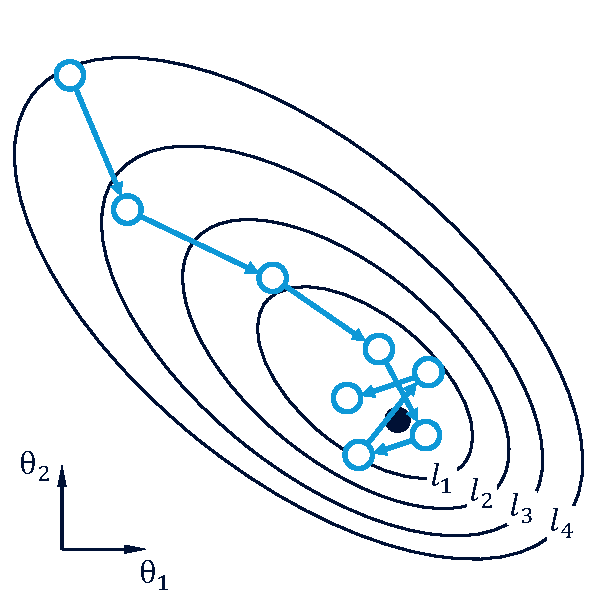
\includegraphics[width=0.4\linewidth]{figures/02_deep_learning/lr_nb/lr_nb_high.pdf}
					\label{fig:lr_nb_high}
				}
				\subfloat[Low $\epsilon$ and $n_b$: slow, erratic but \\ more precise convergence.]{
					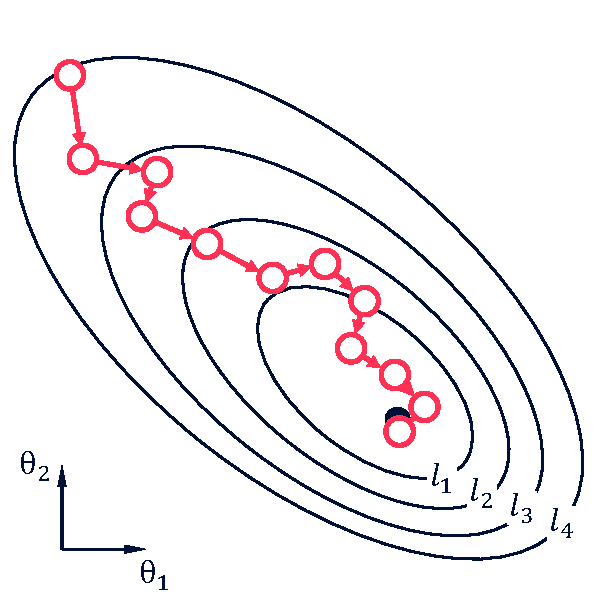
\includegraphics[width=0.4\linewidth]{figures/02_deep_learning/lr_nb/lr_nb_low.pdf}
					\label{fig:lr_nb_low}
				}			
				\caption[Illustration of the effect of different learning rates]{The difference in convergence between high and low learning rate ($\epsilon$) and batch size ($n_b$).}
				\label{fig:lr_nb}
			\end{figure}
			
			In \ac{SGD}, a \emphix{batch}{batch} of input points -- a subset of the whole training set -- is processed at each iteration.
			Stochasticity here refers to the way the batch is assembled: the training points are randomly chosen from the training set, but don't repeat until all training points have been used once.
			The \emphix{batch size}{batch!size} is a user-set parameter.
			A complete round of iterations where every training point was used once is called an \emphix{epoch}{epoch}.
			Most often the duration of training is given in epochs, but sometimes literature also uses the term ``iterations'', which refers to the number of batches propagated in the training.
			Because of the smoothing and robustness increasing effect, larger batch sizes allow for higher learning rates to still converge, but this setup will not converge quite as precisely to the minimum as smaller batches (Fig.~\ref{fig:lr_nb}).
			Smaller batch sizes speed up the computation for a single iteration, but require a smaller learning rate to effectively average out the high variance in the descent over multiple iterations.
			The smaller learning rate also allows for a more precise convergence at the end of the training.
			Naturally, the best of both worlds is to use a large batch size and a low learning rate, however, this can slow down training heavily, requiring a large number of epochs to reach convergence.
			To summarize, the number of epochs, the learning rate, and the batch size all influence \ac{SGD} training in a significant way, and require careful balancing for a robust, but speedy convergence.
			
			Fortunately, users do not have to manually implement any of the above calculations or even the \ac{SGD} training iterations: modern deep learning frameworks automate differentiation and training procedures with simple function calls.
			Deep learning frameworks, such as PyTorch\footnote{\url{https://pytorch.org/}} or TensorFlow\footnote{\url{https://www.tensorflow.org/}}, abstract away most of the complex math, so that new or even long-time users might never have to understand the inner workings of neural net training.
			What users do have to understand, however, are the processing and memory requirements presented by \ac{SGD} and the different metaparameters.
			To realize batched processing, the singular input and output vectors for a \ac{FC} layer in Eq.~\ref{eq:fc_layer} can be changed to $n_b$-tall matrices, resulting in:
			\begin{equation}
				\mathbf{y}_{(n_b \times n_o)} = \mathbf{x}_{(n_b \times n_i)}\mathbf{W}_{(n_i \times n_o)} + \mathbf{b}_{(1 \times n_o)},
			\end{equation}
			\noindent where $n_b$ refers to the batch size, the number of training observations used in this iteration.
			The bias vector $\mathbf{b}_{(1 \times n)}$ is reused in the addition operation for every row of the output matrix, a technique often referred to as \emphix{broadcasting}{broadcasting}.
			
			While this change does not affect the number of parameters that need to be stored, it is clear that both the matrix-multiplication and the addition operations will see an increase in required computations, scaling linearly with $n_b$.
			This is also true for the mostly element-wise operations, such as nonlinearities.
			Furthermore -- as we have seen in Alg.~\ref{alg:gradient_descent} -- the effective implementation of backpropagation requires the storage of intermediate outputs.
			These matrices are quite significant in size, making up the bulk of a neural net's memory footprint during training.
			As all the intermediate output sizes scale linearly with $n_b$, this effectively makes the overall memory requirement of a neural net's training scale linearly with $n_b$.
			In larger nets, or in hardware with limited memory capacity, this scaling often forces the user to utilize smaller batch sizes than optimal.
			This is undesired, because apart from the above mentioned effects on convergence, very small batches can also interfere with some layer's correct functioning, such as batchnorm (Sec. \ref{cha:deep_learning:sec:gradient_stab}).
	
		\subsection{Starting and Stopping, Under- and Overfitting}
			\label{cha:deep_learning:sec:overfitting}
	 
		 	As \ac{SGD} is an iterative optimization, it is sensitive to both starting and stopping conditions.
		 	The starting condition is realized by the \emphix{initialization}{initialization} of the net's parameters.
		 	Net parameters are initialized semi-randomly: the weights are taken from a Gaussian distribution, while the biases are usually initialized to $0$, or very small numbers.
		 	It is important that weights are not initialized to exactly $0$: as can be seen from Alg. \ref{alg:gradient_descent}, a weight of $0$ also blocks the gradient from backpropagating, thereby impeding not only the weight's own training, but every other parameter's training behind it.
		 	In a less obvious way, too small or too large weights are also detrimental to convergence, thus, further refinement is beneficial in the initialization.
		 	We will discuss this topic further in Sec.~\ref{cha:deep_learning:sec:gradient_stab}, but for now, it is enough to have this simple random initialization scheme in mind.
		 	
		 	To be able to tell when a training has converged and when to stop, it is important to discuss the concept of under- and overfitting.
		 	As stated before, neural nets approximate a function.
		 	On one hand this function can be approximated ``lazily'', by not following its curves quite precisely, or in more mathematical terms, the function can be approximated with a less complex function.
		 	If this is the case, yet the neural net could theoretically be able to do better, we talk about \emphix{underfitting}{underfitting}, which occurs mostly because the training stopped too early, or a regularization scheme was used too heavily.
		 	On the other hand, the function to be approximated is only defined in discrete places, where training observations exist.
		 	This leaves the net free to interpolate between the defined points in many ways, possibly using quite complex functions.
		 	If the approximating function is a lot more complex than the theoretically ``correct'' function, we talk about \emphix{overfitting}{overfitting}, which occurs mostly because the net has an overabundance of modeling capacity compared to what the task requires, and the training was not stopped in time.
		 	An illustration of under- and overfitting can be seen in Fig.~\ref{fig:fitting}.
		 	
			\begin{figure}[ht]
				\centering
				\subfloat[Underfitting.]{
					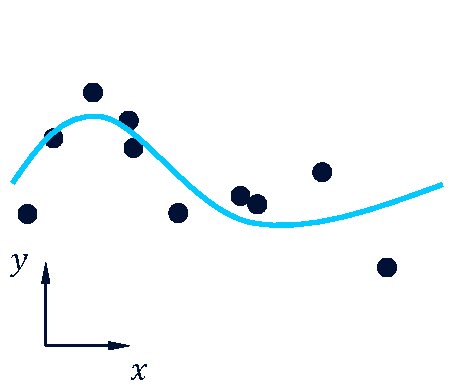
\includegraphics[width=0.3\linewidth]{figures/02_deep_learning/fitting/fitting_under.pdf}
					\label{fig:fitting_under}
				}
				\subfloat[Correct fitting.]{
					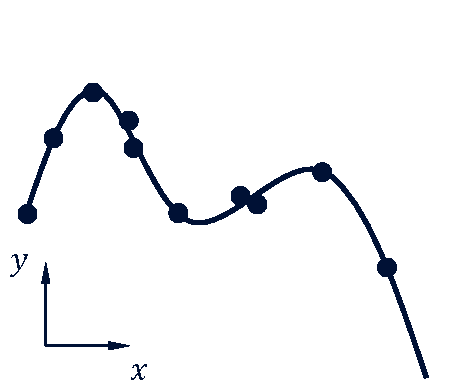
\includegraphics[width=0.3\linewidth]{figures/02_deep_learning/fitting/fitting_correct.pdf}
					\label{fig:fitting_correct}
				}
				\subfloat[Overfitting.]{
					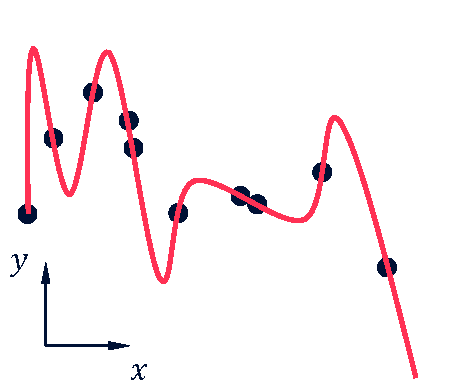
\includegraphics[width=0.3\linewidth]{figures/02_deep_learning/fitting/fitting_over.pdf}
					\label{fig:fitting_over}
				}
				\caption[Over- and underfitting]{Too simplistic, correct and overcomplex function approximations by a neural net.}
				\label{fig:fitting}
			\end{figure}
		 	
		 	Underfitting can be seen as over-generalization: the net is discarding significant variance between the training points, which should be contained within the model.
		 	Similarly, overfitting is under-generalization: the net is learning insignificant variance, in extreme cases formulating rules for individual observations, and losing generalization power in the process.
		 	Neural nets usually learn to approximate a function by moving from an underfitting model towards an overfitting model during their training.
		 	The obvious solution is then to measure how well a net generalizes with its learned rules, and stop the training when the generalization is at maximum.
		 	The idea behind measuring generalization power is that the net cannot overfit observations which it has never encountered during its training.
		 	Furthermore, if a net overfits the training observations and loses generalization power, the learned model will fit these unseen observations quite badly.
		 	To this end, generalization is measured on a \emphix{test}{test!set} or \emphix{evaluation}{evaluation set} dataset, which contains observations that are not included in the \emphix{training}{training!set} set and thus are not used for optimization.
		 	Generalization is usually measured with the same loss function that the training uses, creating the separate \emphix{training loss}{training!loss} and \emphix{test loss}{test!loss}.
		 	
		 	An illustration of how the training and test loss typically develops during a neural net's training can be seen in Fig.~\ref{fig:learning_losses}.
		 	Usually, at the start of the training, both training and test losses decrease, as the net is formulating a more and more complex, but still general model.
		 	Usually, after a while the test loss starts to deviate from the training loss, as non-generic parts of the model start to develop.
		 	However, in these regions, the test loss is usually still decreasing, albeit more and more slowly.
		 	This continues until a point where the test loss starts to increase again, while the training loss keeps decreasing.
		 	The point where the test loss starts to increase is the theoretically best point to stop the training, however, in reality this point is not so straight forward to guess, because usually both losses show a large amount of variance stemming from the stochastic nature of \ac{SGD}.
		 	
			\begin{figure}[ht]
		 		\centering
	 			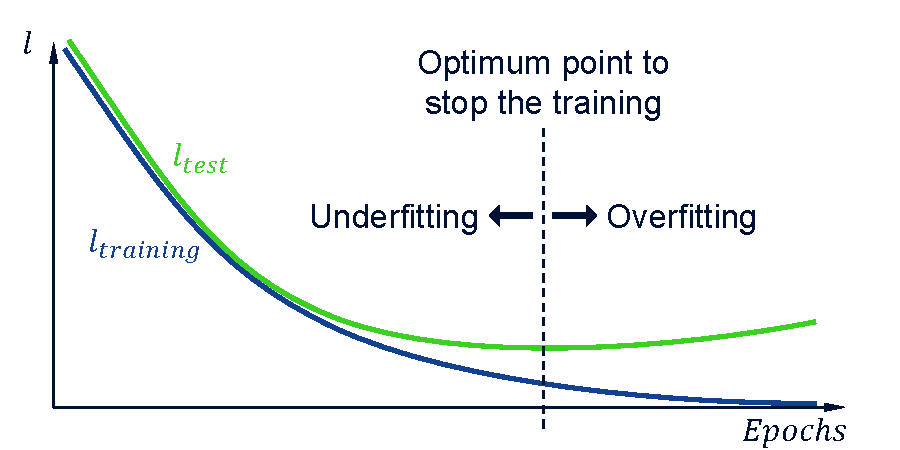
\includegraphics[width=0.6\linewidth]{figures/02_deep_learning/learning_losses/learning_losses.pdf}
		 		\caption[Losses during neural net training]{Typical training and test loss curves during neural net training.}
		 		\label{fig:learning_losses}
		 	\end{figure}
	 	
	 		Another natural way of combating overfitting is to increase the amount and quality of the training data.
	 		By populating all parts of the function-space equally and densely, the ``gaps'' between training points decrease, thereby reducing the freedom of the neural net to interpolate between training points with overtly complex functions.
	 		In another light, because the modeling capacity of the neural net stays the same, increasing the amount of training points reduces the possibility of the net learning individual observations, because there are simply too many to learn.
	 		This highlights the importance of sufficient training data collection, but unfortunately it is not always possible to collect or generate more data if the already acquired set seems insufficient for correct training.
	 		However, reversing the above logic, another way to avoid overfitting is to reduce the complexity of the neural net, which will in turn increase the ``relative'' size of the training dataset compared to the modeling capability of the net.
	 		This can be achieved by pruning the neural net: reducing the number and/or size of the layers.
	 		It is important to be careful when pruning nets, because although this method is very effective in combating overfitting, it is easy to overtly reduce the modeling capacity and thus weaken the potential for a higher accuracy.
	 		
	 		I refer to the previously mentioned methods of early training stopping, large training datasets and limited net complexity as \emphnox{implicit} regularization methods.
	 		I had the most success using these when fine-tuning neural nets.
	 		On the other hand, there also exist \emphnox{explicit} regularization methods, in the form of additional constraints the neural net has to adhere to during training.
	 		I will only mention the most prominent method here: \emphix{weight decay}{weight!decay}.
	 		In this regularization scheme, the learned weights and biases are reduced (decayed) in every iteration by a user-set multiplicative factor which is less than $1$.
	 		This decay has the effect that the net cannot learn overtly large weights which create steep function forms, thus smoothing the approximating function and reducing its complexity.
	 		In my experience, weight decay is tricky to tune, and more often than not hurts both training and test loss, especially when used with adaptive learning rate optimization schemes (Sec.~\ref{cha:deep_learning:sec:gradient_stab}).
			
	\section{Deep Neural Nets}
	
		\subsection{Unstable Gradients in Deep Neural Nets}
		
			Using the previously described \ac{FC} layers followed by sigmoid nonlinearities, we could build a ``traditional'' neural net that is a few layers deep and optimize it with \ac{SGD}.
			For a long time, these shallow neural nets were competitive, but not necessarily better in many tasks than other machine learning algorithms, such as nearest neighbor classifiers, decision trees/forests or \acp{SVM}.
			Although it was recognized early that deeper neural nets would probably be able to learn more complex rules and thus perform better, training any net deeper than a few hidden layers was simply not working.
			Counter-intuitively, increasing the number of hidden layers would often be detrimental to the final accuracy achieved by the net.
			
			The lower accuracy stems from early layers learning slow, thus effectively blocking information from propagating forward to later layers, which in turn slows down the learning of the whole net.
			The more layers these nets have, the more pronounced this effect can be, even going as far as completely preventing the neural net from learning.
			The explanation of this phenomenon is quite straight forward if we look at how the gradients, specifically their amplitude develops layer-by-layer.
			What can be seen in Fig.~\ref{fig:vanishing_gradients} is that the gradients progressively become smaller as they reach the earlier layers of the net.
			This effect is called the \emphix{vanishing gradients}{vanishing gradients} problem, and it is caused by a variety of factors in the net.
			
			\begin{figure}[ht]
				\centering
				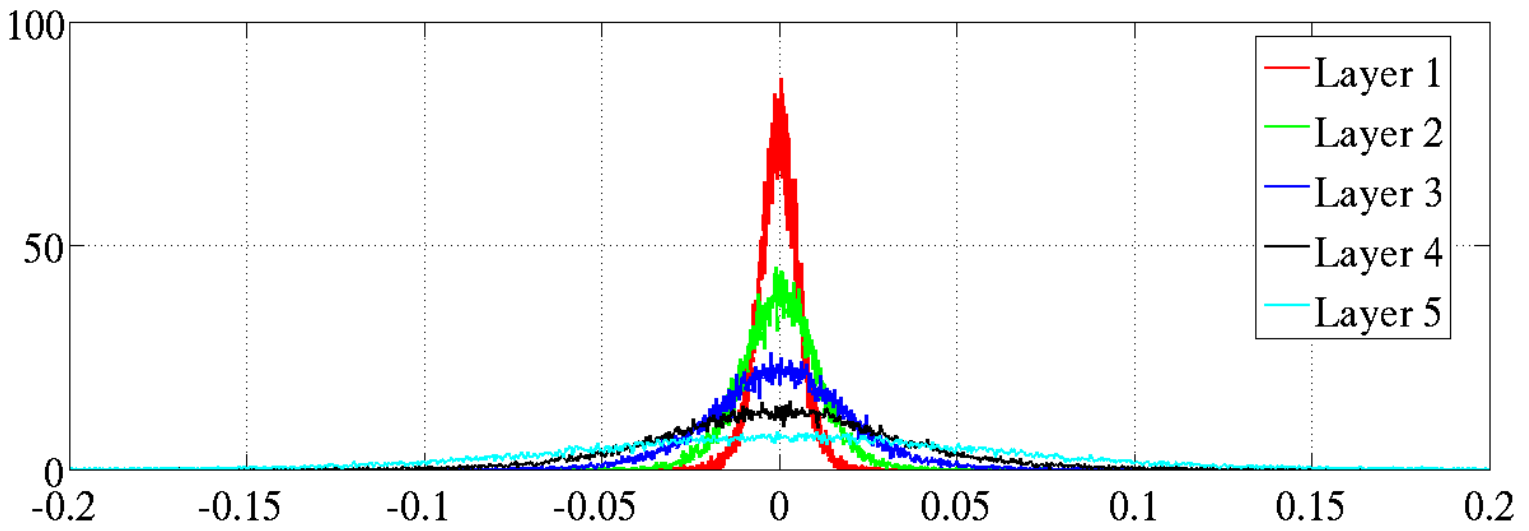
\includegraphics[width=0.8\linewidth]{figures/02_deep_learning/vanishing_gradients/vanishing_gradients.png}
				\caption[Histogram of vanishing gradients]{Histogram of gradients in the first epoch of training in a traditional neural net \cite{deep_net_init}.}
				\label{fig:vanishing_gradients}
			\end{figure}
			
			The biggest factor in vanishing gradients are sigmoid nonlinearities.
			The sigmoid and its related functions have an optimal zone around $0$, where they behave similar to a linear function, and propagate gradients quite well.
			However, even in this zone the derivative is less than $0.25$, thus every sigmoid nonlinearity reduces the gradients to at least $1/4$ (Fig.~\ref{fig:sigmoid_saturation}).
			Outside of this optimal zone, closer to saturation, the derivative of the sigmoid vanishes, thus any gradient propagated backwards through it also tends toward $0$, blocking elements behind from learning.
			While this saturation might make sense if the previous layers ``train into it'' to form learned rules, there is actually no guarantee that the net activations don't end up in saturated regions right at initialization.
			In fact, the more sigmoid layers are present in the net, the larger the chance that the activations will fall on saturated regions somewhere, thus blocking the previous elements from learning.
			
			\begin{figure}[ht]
				\centering
				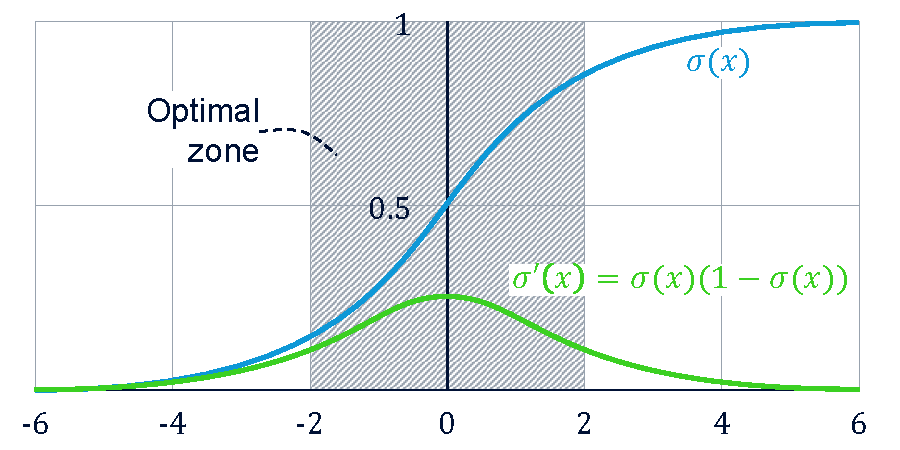
\includegraphics[width=0.6\linewidth]{figures/02_deep_learning/sigmoid_saturation/sigmoid_saturation.pdf}
				\caption[Optimal zone of the sigmoid nonlinearity]{The optimal zone and the derivative of the sigmoid nonlinearity.}
				\label{fig:sigmoid_saturation}
			\end{figure}
		
			To counteract this, one could try to center the activations at initialization, so that most sigmoid nonlinearities receive inputs around $0$, by initializing \ac{FC} layer weights to small numbers.
			However, as shown in Alg.~\ref{alg:gradient_descent}, backpropagating gradients through an \ac{FC} layer means multiplying the gradient by the transpose of the weight matrix.
			If the weights are small numbers, this multiplication will severely reduce the gradients, possibly much more so than the sigmoid nonlinearity could.
			On one hand, this highlights the fact that depending on the weight initialization, \ac{FC} layers can also be a contributing factor in the vanishing gradients problem.
			On the other hand, it seems it would be possible to counteract the gradient-reducing effects of the sigmoid nonlinearities by ``restoring'' the gradients with larger weights in \ac{FC} layers.
			However, large initial weights can quickly lead to the opposite of the vanishing gradients problem: \emphix{exploding gradients}{exploding gradients}.
			If \ac{FC} weights are big enough to have a gradient-increasing effect, backpropagating gradients through multiple such \ac{FC} layers can create exponentially large gradients in early layers.
			This can lead to these layers not being able to learn, thus once again blocking information from reaching later layers and hurting or completely stopping the learning in the whole net.
			
		\subsection{Stabilizing Gradients}
			\label{cha:deep_learning:sec:gradient_stab}
	
			From the previous discussion, we can conclude that gradients are inherently unstable.
			The key to training deep neural nets is then to stabilize gradients, so that earlier layers are also able to learn and thus propagate valuable learned features to later layers.
			This stabilization is not achieved through a single trick, rather, the constant mitigation of vanishing and exploding gradients, which incorporates many elements in the net.
			As one of the biggest factors in vanishing gradients are the sigmoid nonlinearities, we can start by stabilizing the gradient using a better nonlinearity.
			
			A key aspect of the sigmoid nonlinearity is its bounded output.
			This boundedness ultimately forces the function to saturate, and the derivative to vanish, causing propagated gradients to also reduce or completely vanish.
			However, there is no clear reason why nonlinearities need to be bounded in either direction.
			\emphix{\ac{ReLU}}{rectified linear unit} nonlinearities do not adhere to this criteria, by realizing a simple function which is the identity on positive inputs, and a small multiplier on negative inputs, i.e.:
				
			\begin{figure}[ht]
				\centering
				\begin{minipage}[t]{0.5\linewidth}
					\begin{equation}
					\label{eq:relu}
					f_{ReLU}(x_j) = \begin{cases}
					x_j & if\; x_j > 0 \\
					\alpha{x_j} & if\; x_j < 0
					\end{cases},
					\end{equation}
				\end{minipage}
				\begin{minipage}[t]{0.3\linewidth}
					\raisebox{-0.8\height}{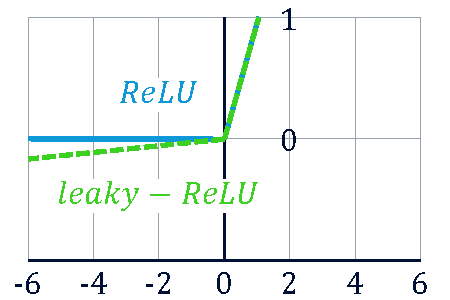
\includegraphics[width=\linewidth]{figures/02_deep_learning/nonlins/relus.pdf}}
				\end{minipage}
				\caption[ReLU and leaky-ReLU nonlinearities]{ReLU and leaky-ReLU nonlinearities.}
				\label{fig:nonlins_relus}
			\end{figure}
			\noindent where $\alpha$ is a small number, representing the ``leakyness'' (slope) of the negative part of the function. 
			
			\ac{ReLU} has a very simple derivative:
			\begin{equation}
				\frac{\delta}{\delta{x_j}} f_{ReLU}(x_j) = \begin{cases}
					1 & if\; x_j > 0 \\
					\alpha & if\; x_j < 0
				\end{cases}.
			\end{equation}
			\noindent The derivative of $1$ on the positive parts does not scale the backpropagated gradients, which helps greatly in stabilization.
			\ac{ReLU} was defined originally as $\alpha = 0$, but it was soon realized that the $0$ derivative can often cause neurons or whole parts of the net to get ``stuck'' right after initialization.
			\emphix{Leaky-\ac{ReLU}}{leaky rectified linear unit} solves this by giving a slight slope to the negative parts, thus allowing for training even if the activations happen to fall to the negative range at initialization, allowing for the net to train ``out'' of a bad initialization.		
			
			As discussed, the second most important factor in the unstableness of gradients are \ac{FC} layer weights.
			It is impossible to avoid any gradient degradation throughout the whole training, because the nets learn and formulate rules by changing these weights.
			However, at least the initialization can be done so that gradients are stable in the first few iterations.		
			Most advanced initialization schemes assume a distribution of activations on the \ac{FC} layer inputs, and aim to initialize weights so that this distribution is retained after the following nonlinearity, as input for the next \ac{FC} layer.
			Naturally, this makes the initialization schemes specific to the nonlinearity used.
			By keeping the distribution of the activations the same throughout the net, statistically speaking the combined \ac{FC} and nonlinearity layer pairs don't scale the activations, thus also keeping the gradients stable (Fig.~\ref{fig:normalized_gradients}).
			The weight initialization is usually done in the previously described manner, by randomly generating weights from a Gaussian distribution, however, advanced schemes scale the generated weights to a certain variance as a second step.
			The most famous such scheme is the \emphnox{Xavier} initialization \cite{deep_net_init}, which is defined for tangent-hyperbolic nonlinearities.
			For \ac{ReLU} nonlinearities, the \emphnox{He} initialization can be used \cite{deep_net_init_relu}.
			
			\begin{figure}[ht]
				\centering
				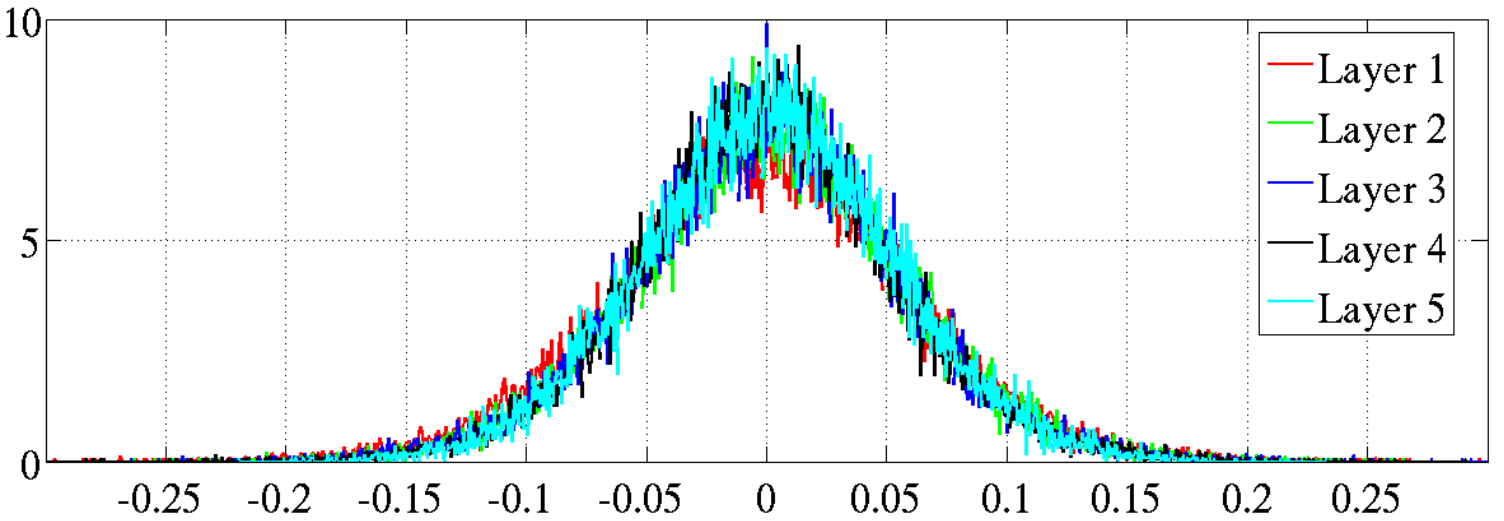
\includegraphics[width=0.8\linewidth]{figures/02_deep_learning/normalized_gradients/normalized_gradients.png}
				\caption[Histogram of stabilized gradients]{Histogram of stabilized gradients using the Xavier initialization \cite{deep_net_init}.}
				\label{fig:normalized_gradients}
			\end{figure}
		
			Advanced optimization schemes also play an important role in facilitating the training of deep neural nets.
			All of these optimization schemes are still \ac{SGD}- and backpropagation-based, but do not simply update the weights with a preset learning rate, rather, additional factors play a role.
			The first major advancement in optimization schemes was the addition of \emphix{momentum}{momentum}.
			Momentum implements a physical analogy in the weight updates, where the previous weight updates are taken into account in the current update using an exponential decay.		
			This is similar to the Newtonian dynamics of a ball rolling down a hill (the loss surface) and not stopping when encountering bumps or saddle points due to inertia.
			Momentum can smoothen and speed up \ac{SGD} training, as well as mitigate the vanishing gradients problem by accumulating small gradients into the inertia, thus allowing for effective training even if the gradients are close to vanishing.
			However, the biggest mitigation for vanishing or even exploding gradients are \emphix{adaptive learning rate}{adaptive learning rate} optimization schemes.
			Adaptive learning-rate optimization algorithms effectively mitigate a lot of the downsides of \ac{SGD} stemming from its iterative and greedy nature (as outlined in Sec.~\ref{cha:deep_learning:sec:sgd_backprop}).
			In these, each parameter is updated using an individual learning rate, which is automatically set in order to normalize the first and/or second order moments of the weights.
			The most recent such advanced optimization scheme -- and the one I had the most success with -- is \emphix{\ac{Adam}}{adam} \cite{adam}.
			\ac{Adam} combines momentum with adaptive learning rates, by scaling individual learning rates with their first and second order moments.
			\ac{Adam} is capable of robustly training deep neural nets where any other optimization scheme fails.	
			
			Lastly, the \emphix{batchnorm layer}{batchnorm layer} is often used to explicitly normalize activations and thus gradients in the net \cite{batchnorm}.
			As the name implies, batchnorm layers normalize -- scale and center -- activations per batch, but often also contain trainable parameters with which the net can learn to ``undo'' this normalization to a degree:
			\begin{equation}
				\mathbf{y} = \frac{\mathbf{x} - E_{n_i}(\mathbf{x})}{\sqrt{Var_{n_i}(\mathbf{x})}}\gamma + \beta
			\end{equation}
			\noindent where $E_{n_i}(\mathbf{x})$ refers to the per-dimension batch-wise mean of the input batch $\mathbf{x}_{(n_b \times n_i)}$, $Var_{n_i}(\mathbf{x}$ to the per-dimension variance of the same, $\gamma$ to a learnable scaling and $\beta$ to a learnable offset parameter.		
			Although excellent for normalizing activations, batchnorm layers also add a certain amount of random variance into the system, because of the stochasticity contained in each batch.
			The added variance increases inversely to the batch size, so it is not recommended to use batchnorm layers with extremely small batches, as this could disturb the neural net training.
			Batchnorm layers can also function differently during inference, when the batch-wise mean and variance is not calculated, rather, stored values are used which were learned during training.
			
			With all these elements combined, it is now quite possible to train very deep neural nets, which contain \ac{FC} layers numbering in the hundreds.
			However, nowadays most deep neural nets are not made up of \ac{FC} layers, rather, specialized layers are used in order to realize specific tasks, such as sequence processing or image recognition.
			
		\subsection{Recurrent Nets}
			\label{cha:deep_learning:sec:recurrent_nets}
		
			\emphix{\acp{RNN}}{recurrent!neural net} extend on the traditional neural net concept by incorporating the \emphnox{temporal} context of the information -- such as in written text or in a time-series -- by processing it in a sequential order, one observation at a time.
			\acp{RNN} are made up of \emphix{recurrent layers}{recurrent!layer} (also called recurrent cells).
			These layers utilize a hidden state $h_t$, which is also the output of the recurrent layer, that feeds back to the input at every step of the sequence, retaining a \emphnox{memory} of all previous states (Fig.~\ref{fig:rnn_rnn}). 
			The hidden state $h_t$ includes all atomic states from every neuron, and is also fed back to every one of them, so that each neuron gains access to all neuron’s hidden states in the same cell. This hidden state can be described by the equation:
			\begin{equation}
				\mathbf{h}_t = f_{nonlin}(\mathbf{x}_t\mathbf{W} + \mathbf{h}_{t-1}\mathbf{U})
			\end{equation}
			\noindent where $h_t$ is the hidden state at step $t$, $x_t$ is the input vector, and $W$ and $U$ are fully-connected weight matrices.
			At every step, the recurrent cell not only receives the input of the current step ($x_t$), but concatenated to it is also the previous output (hidden state).
			This creates a feedback loop, enabling the net to make decisions based not only on the current input, but also on past states.
			
			\acp{RNN} typically have a relatively low number of cells, compared to the number of layers in other modern deep neural nets.
			However, \acp{RNN} should still be categorized as deep nets; when processing the sequence, a single recurrent layer can be imagined as a repeated sequence of layers, each processing as input the corresponding historical timestep and feeding its output into the next layer.
			The depth of recurrent nets comes from the fact that this “unrolled” net can be very large, depending on the length of the input sequence.
			Due to this, in most cases it is wise to limit the number of the actual recurrent layers in a neural net, since the sequential nature of the net already introduces vast complexity.
			Furthermore, when backpropagating, the derivatives should theoretically be unrolled in time all the way to the first input, however, this would cause an intractable memory footprint for these algorithms.
			To overcome this, \acp{RNN} use a truncated backpropagation implementation, which only unrolls gradients until the last $k$ user-defined steps.
			
			\begin{figure}[ht]
				\centering
				\subfloat[Simple RNN cell]{
					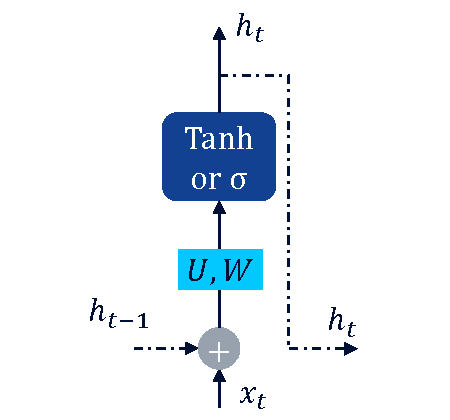
\includegraphics[width=0.3\linewidth]{figures/02_deep_learning/rnn/rnn.pdf}
					\label{fig:rnn_rnn}
				}
				\subfloat[LSTM cell]{
					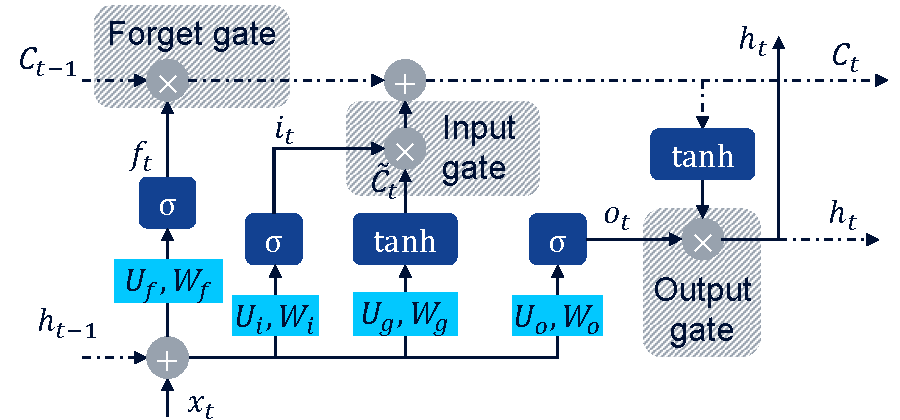
\includegraphics[width=0.6\linewidth]{figures/02_deep_learning/rnn/lstm.pdf}
					\label{fig:rnn_lstm}
				}
				\caption[Recurrent cells]{Recurrent cells.}
				\label{fig:rnn}
			\end{figure}
			
			In this simple form, \acp{RNN} are notoriously prone to vanishing or exploding gradients.
			Because of their recursive nature, the activations pass through the same weights multiple times, which also means the gradients also have to be backpropagated through the same weights multiple times.
			If the weights amplify or dampen the gradients even just a little, this repeated backpropagation can quickly lead to exploding or vanishing gradients.		
			A successful architecture that overcomes these unstable gradients is the \emphix{\ac{LSTM}}{long short-term memory} cell \cite{lstm}.
			\ac{LSTM} cells deal with vanishing gradients by introducing an internal memory ($C_t$), that is not the same as the cell’s output.
			This internal memory is governed by a complex layout of input-, output- and forget-gates in the cell (Fig.~\ref{fig:rnn_lstm}).
			The forget-gate keeps or clears the internal state based on the input and the previous hidden state. 
			The input-gate regulates how much of the new input is added to the internal state, while the output is a version of the new internal state filtered by the output-gate.
			Intuitively, the \ac{LSTM}’s various gates regulate how much the \ac{RNN} takes the past and new information into account, only considering the most useful inputs instead of using all the past timesteps with decreasing weight as it is in simple \acp{RNN}.
			This also helps to overcome the unstable gradient problem; the \ac{LSTM} cell is able to compensate for exploding or vanishing gradients through these gates by avoiding the propagation of the same gradient multiple times through the same weights, even between timesteps in the same input sequence.
			
			Today’s \acp{RNN} target variable-length sequence processing tasks, mainly in the field of \ac{NLP}.		
			Natural languages are composed of a hierarchical structure of sentences, expressions, words and finally letters or sounds. 
			This multi-level representation can be learned using \acp{RNN}, by stacking multiple \ac{LSTM} layers, similar to the way other deep neural nets build up their hierarchical feature representations; earlier layers learn lower level features (in this case words), while later layers learn high level representations (sentences).
			\ac{LSTM} layers are especially powerful for \ac{NLP} tasks, because in languages the dependencies in time can vary greatly: for example, some conjugations only depend on the immediate word they are appended to, while other conjugations can depend on words which are whole sentences away.
			However, as the premier sequence-processing deep nets, \acp{LSTM} are also often used for much simpler, fixed-length sequences with a less hierarchical structure, mostly only because of their fame.
			The question remains then if recurrent nets are truly the best tool for processing such sequences.		
	
		\subsection{Convolutional Nets}
			\label{cha:deep_learning:sec:convolutional_nets}
		
			\emphix{\acp{CNN}}{convolution!-al net} extend on the traditional neural net concept by incorporating the \emphnox{spatial} context of the information, such as in images or heatmaps, by paying attention not only to the value of the features, but also to the value of neighboring features and their relative position \cite{cnn}.
			\acp{CNN} are made up of convolutional layers, which realize the mathematical operation of \nomphix{convolution}{convolution} between the input \emphix{tensors}{tensor} ($n$-dimensional matrices) and learned filters.
			Convolution is originally defined as a mathematical operation on two functions, which computes the amount of overlap of one function as it is shifted over the other.
			In $1$-dimension, convolution may be visualized as sliding one function, $f$ (\nomphix{filter}{filter}), on top of another, $g$ (input), while, at each shift, point-wise multiplying the functions and adding the products as illustrated in Fig.~\ref{fig:convolution}.
			
			\begin{figure}[ht]
				\centering
				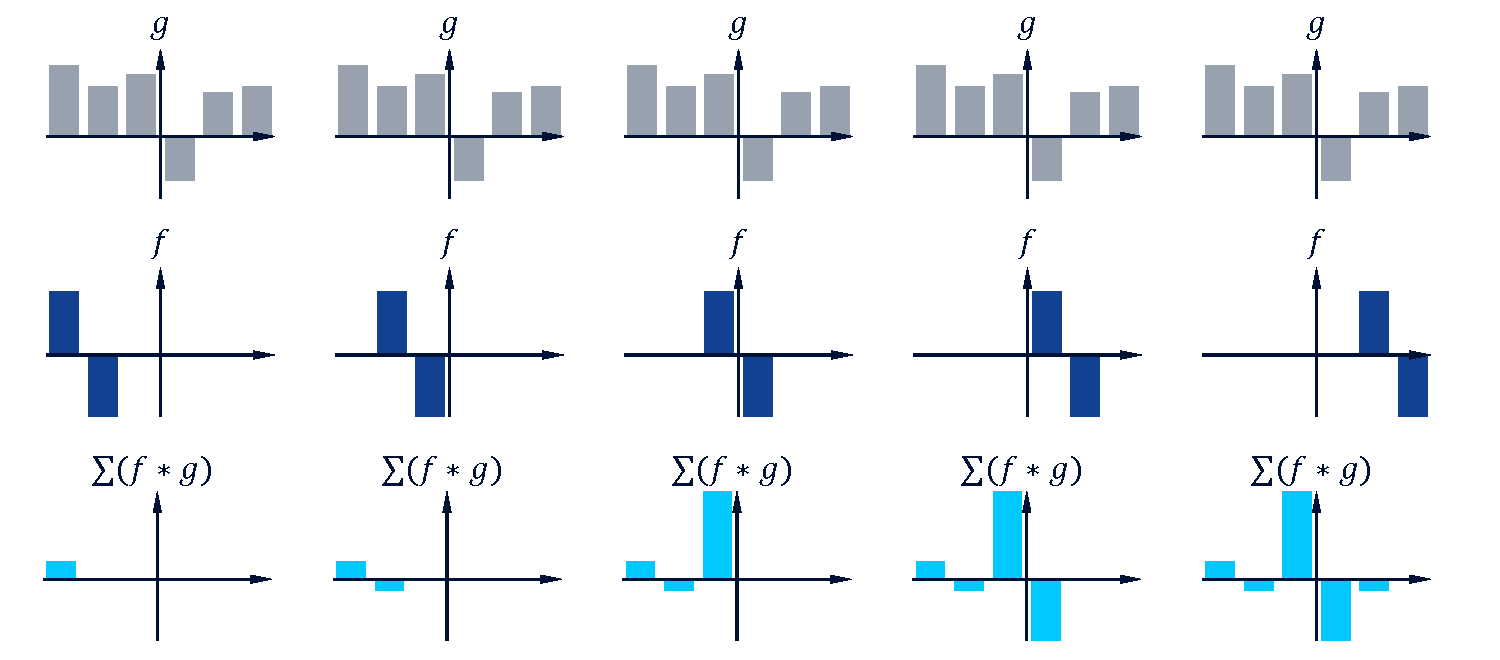
\includegraphics[width=\linewidth]{figures/02_deep_learning/convolution/convolution.pdf}
				\caption[Convolution of two functions]{Convolution of two functions.}
				\label{fig:convolution}
			\end{figure}
		
			The convolution operation can be trivially extended to multiple dimensions, where the input, the filter and the output tensor of the operation will always be the same dimensionality in the convolution dimensions.
			Most often, \acp{CNN} are used for image-like data, thus, the convolution is $2$-dimensional.
			In these cases, the input and the output is a $3$-dimensional tensor where the first $2$ dimensions ($x$ and $y$, or width and height) correspond to the plane of the original image and define the location of activations for the same filter output, while the $3^{rd}$ dimensions ($z$, or depth) incorporates the outputs of different filters.
			The $z$ dimensions are also often referred to as channels, such as the red, green and blue channels in color images.
			
			\emphix{Convolutional layers}{convolution!-al layer} are made up of small filters (such as a $3\times3\times{z}$ grids), each reacting when detecting a unique structure.
			This detection is done through the usual matrix multiplication also used in fully connected layers; the filters are learned weights, which are multiplied by a part of the input tensor and then summed to form a single output value.
			The filters scan the output of the previous layer in the $x$ and $y$ dimensions step-by-step, and produce an output tensor, which contains the localized activations of the filter for each scanned position.
			The filters' receptive area usually extends through the whole depth ($z$) of the previous output tensor.
			
			\begin{figure}[ht]
				\centering
				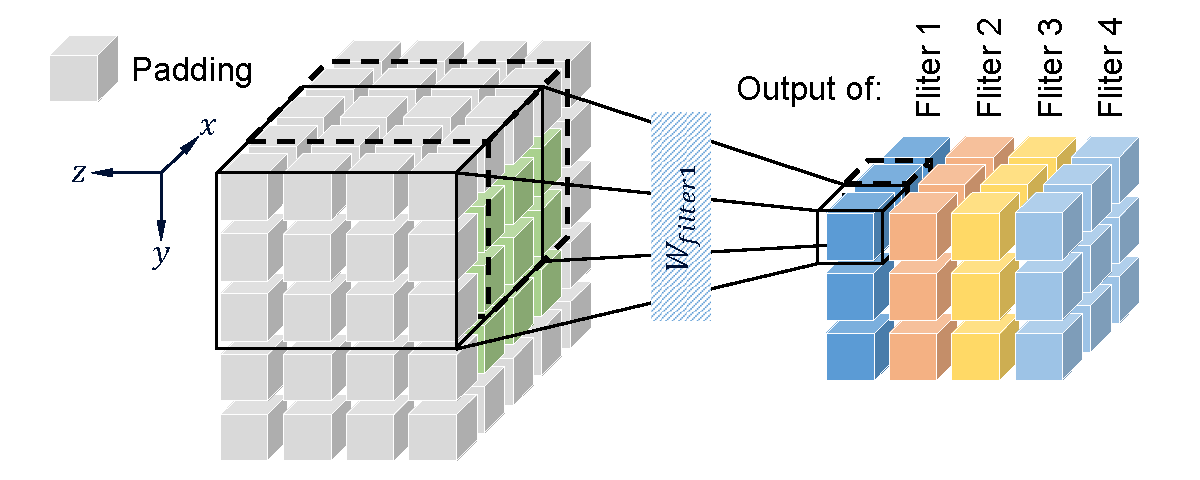
\includegraphics[width=0.8\linewidth]{figures/02_deep_learning/conv_layer/conv_layer.pdf}
				\caption[Convolutional layer]{Illustration of a $2$-dimensional convolutional layer, its input and output tensors.}
				\label{fig:conv_layer}
			\end{figure}
		
			The size of the output of these layers is governed by multiple parameters: the actual filter size, the number of filters, the stride (the step size of the scan) and the amount of padding on the sides of the previous output.
			The example in Fig.~\ref{fig:conv_layer} illustrates a convolution on a $3\times3\times4$ tensor with a padding of $1$, using $4$ different $3\times3\times4$ filters with a stride of $1$.
			Often, convolutional layers pad the input tensor, in order to retain the same output tensor shape as the input.
			There are various padding strategies, the most often used are $0$-padding and mirror padding.
		
			The convolutional filters are receptive to spatial structures, realizing a sensitiveness to position in their inputs, and encode the position of the sensed features in their output.
			\acp{CNN} often utilize \emphix{pooling layers}{pooling layer}, which undertake the conceptually opposing task; their job is to mitigate the strong sensitiveness of the convolutional layers with regards to exact position or orientation.
			They do this with a scanning compression method similar to the filters in the convolution layer, but only propagating the largest (max-pooling) or the average (average-pooling) activation value from a small area of the input, thereby also scaling down (compressing) the propagated tensors in the convolution dimension. 
			The compression areas are restricted to a depth of $1$, and are usually small, $2\times2$ or $3\times3$ in the x-y plane.
			The stride of the scan can be either set to create overlapping or non-overlapping scans, however, usually non-overlapping pooling is used.
			An example of max-pooling is illustrated in Fig.~\ref{fig:pooling_layer} with a $2\times2$ compression area and no overlap.
			
			\begin{figure}[ht]
				\centering
				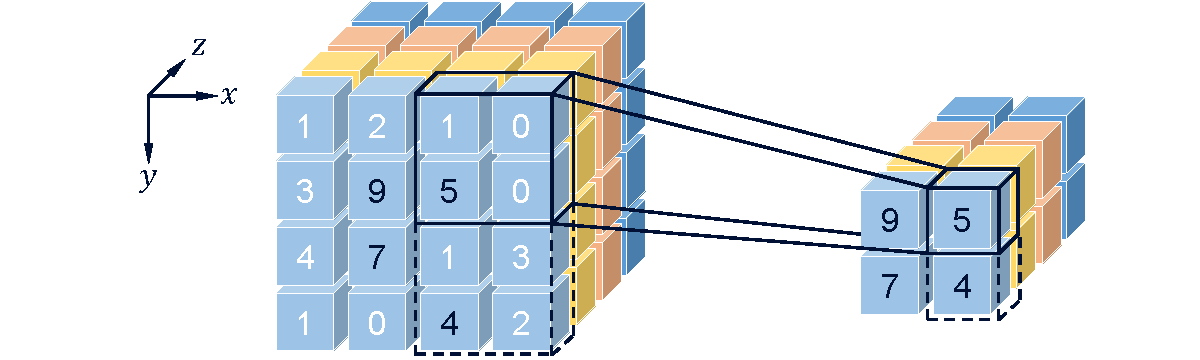
\includegraphics[width=0.8\linewidth]{figures/02_deep_learning/pooling_layer/pooling_layer.pdf}
				\caption[Max-pooling layer]{Illustration of a $2$-dimensional max-pooling layer, its input and output tensors.}
				\label{fig:pooling_layer}
			\end{figure}
			
			Pooling enforces sparsity in the inner representation of the net, acting as a regularizer, and compressing information.
	 		Overall, this regularization manifests as an insensitivity to the exact orientation, skew or position of the objects in the input image, which is a sought-after property for robust and precise recognition.
			Max pooling also combats the vanishing gradient problem by only routing the gradient to the most activated position in the previous layer.
			This avoids splitting the gradient into multiple parts, which in turn avoids the repeated gradient division present in fully connected layers.
			
			It is important to note that the convolution operation could also be realized with a simple fully connected layer.
			In fact, convolutional layers can be viewed as fully connected layers that have connections which are turned off, and others that share weights across the layer, as depicted in Fig.~\ref{fig:fc_conv}.
			This view highlights the original aim of the convolutional layer; to reduce the number of weights in the net by leaving out often unused parts, so that deeper, more complex nets could be fit into state-of-the-art hardware.
			Convolutional and pooling layers are often used for image processing, but are not solely useful for those tasks.
			$1$-dimensional convolutions can also be useful for fixed-length sequence processing, while $3$-dimensional convolutions could be capable of processing heatmaps, such as coverage maps with the temporal context also taken into account.
			
			\begin{figure}[ht]
				\centering
				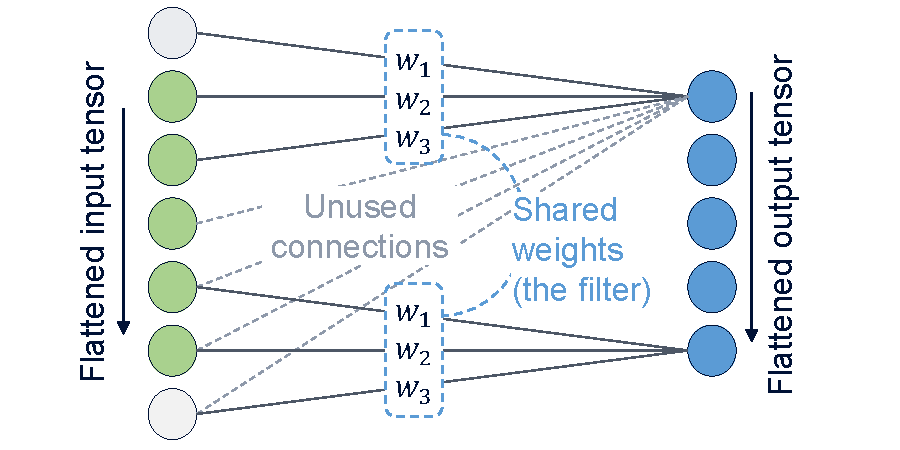
\includegraphics[width=0.6\linewidth]{figures/02_deep_learning/fc_conv/fc_conv.pdf}
				\caption[Derivation of a convolutional layer from an FC layer]{Derivation of the convolutional layer from the FC layer, through unused connections and shared weights.}
				\label{fig:fc_conv}
			\end{figure}
			
		\subsection{Autoencoders}
			\label{cha:deep_learning:sec:ae}
		
			\emphix{\acp{AE}}{autoencoder} are a set of neural net architectures, used to form an abstract latent representation of the data through unsupervised learning.
			Autoencoders are made up of an \textit{encoder} and a \textit{decoder} subnet, which are usually mirror-equivalents of each other.
			The role of the encoder subnet is to learn to ``encode'' information about the training observations into a constrained space, while the decoder has to learn to reconstruct the original observations using this information.
			Traditional autoencoders compress data, all the while minimizing the loss of relevant information, making use of the fewer but more abstract internal features formed in the middle layers.
			The measure of goodness for an autoencoder is how well it can restore the original data from its internal representation, which is usually calculated as the \ac{MSE} between the input and the output of the net. 
			The goal of compression is immediately visible in the topology of an autoencoder; the nets narrow up to the middle layers, then widen again to regain the same width as the input layer (Fig.~\ref{fig:autoencoder}).
			This topology forces the net to form higher abstractions in the middle layers, causing irrelevant or redundant information not to be propagated.
			
			\begin{figure}[ht]
				\centering
				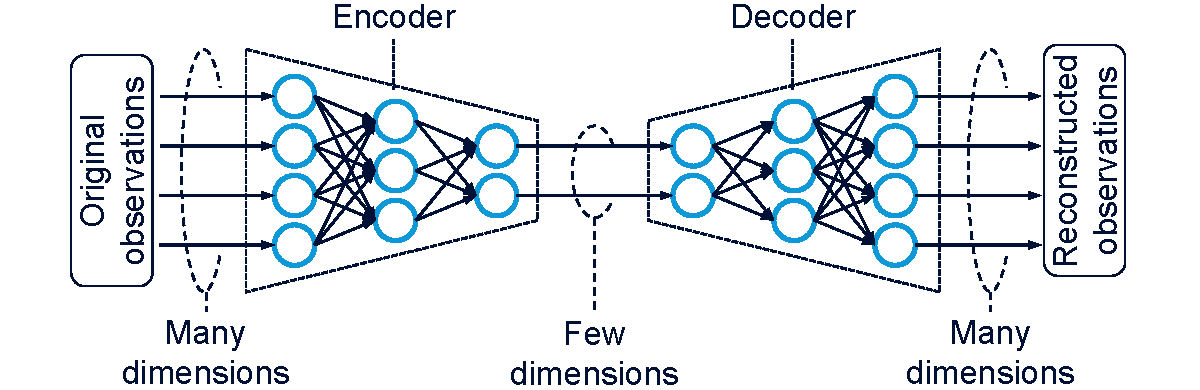
\includegraphics[width=0.8\linewidth]{figures/02_deep_learning/autoencoder/autoencoder.pdf}
				\caption[Traditional autoencoder architecture]{Traditional autoencoder architecture.}
				\label{fig:autoencoder}
			\end{figure}
			
			A specific type of autoencoder we often utilized often in our research is the \emphix{convolutional autoencoder}{convolution!-al autoencoder}.
			In this, instead of the usual \ac{FC} layers, the encoder employs convolutional and pooling layers, however, to retain symmetry, the decoder has to utilize special deconvolutional and unpooling layers.	
			\emphix{Deconvolutional layers}{deconvolutional layer} realize a mirrored convolution: the filters expand singular input values into larger tensors in the output.
			Similarly, \emphix{unpooling layers}{unpooling layer} also reverse the pooling operation by scaling up the inputs.
			The inverse operation of average pooling is simply upscaling, where the same input value is repeated over the whole output area.
			However, the inverse operation of max-pooling is not that straight forward: in this case, the output area is filled by $0$s in all except one position, where the input value is placed.
			In order to know which position this value has to be placed, the maximum location indices have to be saved in the symmetrical max-pooling layer in the encoder, and communicated to the max-unpooling layer in the decoder.
			
			Autoencoders are the earliest deep neural net architectures, preceding the technological and algorithmic advancements that allowed for the training and use of modern deep neural nets.				
			The reason why autoencoders were still possible to train - avoiding vanishing gradients and not requiring enormous computational power - is because of the greedy, layer-by-layer training method they implemented. 
			These \emphix{stacked autoencoders}{stacked autoencoder} start with only the outer layers present, and add layers by pairs to the middle of the autoencoder, only after the previous net has reached convergence.		
			This method limits the calculations to a few layers at any time, allowing for deep nets to be trained on less capable hardware.
			At the end of the training, the weights could be fine-tuned with end-to-end backpropagation; at this point vanishing gradients do not pose a big threat to the net. Nowadays this training method has fallen out of favor, as gradient stabilization methods and hardware-accelerated computations made the training of deeper autoencoders in an end-to-end fashion possible from the start.
		
		\subsection{Generative Adversarial Nets}
			\label{cha:deep_learning:sec:gan}
		
			\emphix{\acp{GAN}}{generative adversarial net} are a neural net architecture and training paradigm, which is focused on the generation of entirely synthetic, albeit believable data points \cite{gan}.
			In their simplest form, \acp{GAN} are made up of a \emphix{generator}{generator} and a \emphix{discriminator}{discriminator} subnet.
			\acp{GAN} use an adversarial training method in which, during training, the two subnets are assigned opposing tasks: the generator has to learn to generate synthetic observations from points sampled randomly from a user-defined distribution, which are indistinguishable from real observations, while the discriminator has to try to distinguish the synthetic observations from real observations (Fig.~\ref{fig:gan}).
			
			\begin{figure}[ht]
				\centering
				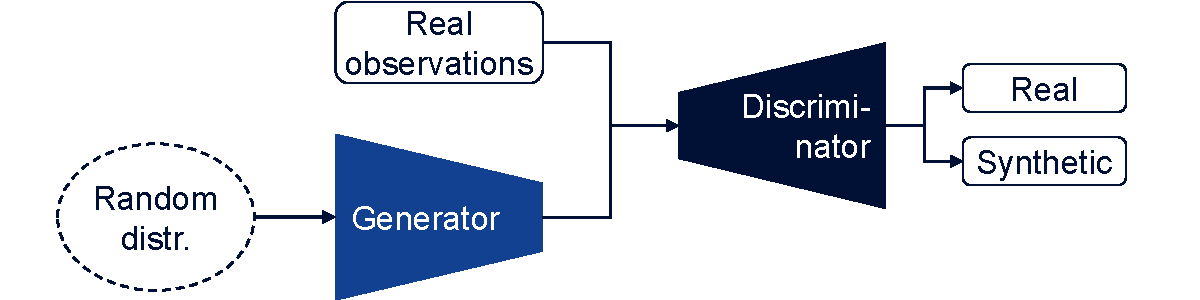
\includegraphics[width=0.8\linewidth]{figures/02_deep_learning/gan/gan.pdf}
				\caption[GAN architecture and training]{Generative adversarial net architecture and training.}
				\label{fig:gan}
			\end{figure}		
			
			This objective can be seen as an adversarial zero-sum game that the two subnets are playing.
			Naturally, because of the adversarial nature, the training of these nets is quite chaotic, so often there are external regularizing factors in-place which guide the nets towards their correct objective.
			The end goal of the game is for the generator to ``win'', by learning to generate convincing observations that are indistinguishable from real observations by the discriminator.
			After training, the discriminator can be discarded, and the generator used to generate synthetic observations by supplying it with random inputs taken from the user-defined distribution.		
			In reality, the adversarial training realized by the discriminator actually forces the generator to learn to output the same \emphnox{distribution} as is present in the training data.
			This matching of distributions is useful for other simpler tasks too, such as enforcing a distribution in the middle of an autoencoder.
			
		\subsection{Hierarchical Features Learned in Deep Neural Nets}
			\label{cha:deep_learning:sec:hierarchical_features}
			
			The quick spread of use and acknowledgment of deep learning cannot be tied to a single invention, but rather to multiple smaller factors that together enabled the training and use of deep neural nets, what is today referred to as deep learning.
			Correspondingly, there is a lot of misuse of the term, stemming from misconceptions about what does and does not constitute as deep learning.
			However, there is no breaking point, no set number of hidden layers above which one can call a net deep.
			As such, instead of defining deep learning by the applied number of hidden layers, it is necessary to find a definition that is also applicable outside the realm of neural nets, and instead focuses on what is achieved by deep learning.
			The first \acp{DNN} performed better than their non-deep predecessors because they could learn complex, hierarchical rules or features present in the training data.
			This deep understanding is what defines whether a system achieves deep learning.
			
			This section is meant as a practical summary of the many elements of deep learning discussed so far, and as an illustration of the hierarchical features learned by \acp{DNN}.
			For this, we can look at the famous VGG16 neural net topology \cite{vgg16}, which achieved top results in the \ac{ILSVRC} in $2014$\footnote{\url{http://www.image-net.org/challenges/LSVRC/2014/results}}.
			\ac{ILSVRC} is an image recognition challenge, where the submitted machine learning algorithms have to correctly identify the class of the image out of a $1000$ categories, which include photographs of objects and different kinds of animals.
			It was at \ac{ILSVRC} where the first deep neural nets were introduced, and winning the challenge it still held as one of the biggest achievements one can make in the \ac{DL} field. 
			VGG16 is a truly deep neural net, employing $16$ convolutional and \ac{FC} layers, followed by batchnorm layers and \ac{ReLU} nonlinearities, max-pooling layers, and a softmax nonlinearity at the output.
			The topology can be seen in Fig.~\ref{fig:vgg16_topo}, which depicts the output tensor shapes of the layers in the net.
			
			\begin{figure}[ht]
				\centering
				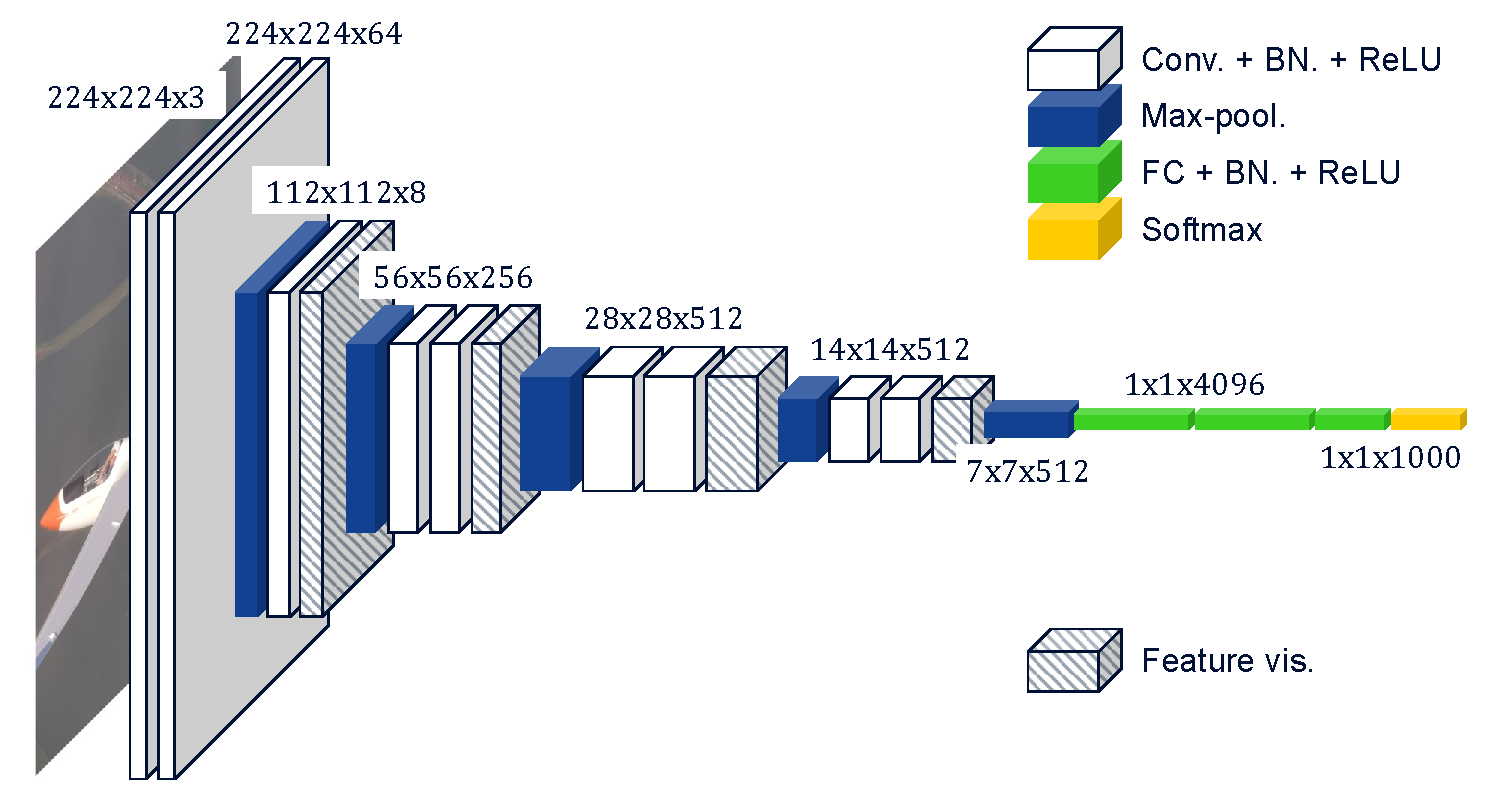
\includegraphics[width=\linewidth]{figures/02_deep_learning/vgg16_topo/vgg16_topo.pdf}
				\caption[VGG16 topology]{Topology of the VGG16 net.}
				\label{fig:vgg16_topo}
			\end{figure}
			
			To gain better insight into how \acp{DNN} learn, techniques were developed which visualize the features learned by the different neurons in the net.
			The visualizations I show can be achieved with the very same tools that are used to train the net\footnote{\url{https://distill.pub/2017/feature-visualization/}}: here, instead of the net parameters, gradient descent is used to optimize the \emphnox{input image} itself, in order to best trigger a specific neuron.
			The process requires a skew of regularization methods to produce nice looking images, such as step-by-step upscaling of the image, as well as constant random transformations such as small rotations and translations, in order to avoid very noisy images and to aid in the formulation of larger features.
			Tuning these to produce nice images is an art in itself.
			I generated such visualizations from different layers of the pretrained VGG16 net.
			The hierarchical features learned by the net are quite nicely illustrated (Fig.~\ref{fig:feature_vis_layers}): neurons in earlier layers are triggered by simpler shapes, such as edges or textures, while later layers are triggered by more complex structures.
			Finally, visualizations from the very last layer create images of the different object categories the net was trained to recognize, which contain, in a dream-like collage, all the most important aspects of the object category in question (Fig.~\ref{fig:feature_vis_classes}).
			I think these images are best kept in mind when discussing deep learning, as one should always be critical in any given task whether such hierarchical features can be learned from the data, and thus whether using deep learning is warranted.
			
			\begin{figure}[ht]
				\centering
				\subfloat[Layer $11$: textures.]{
					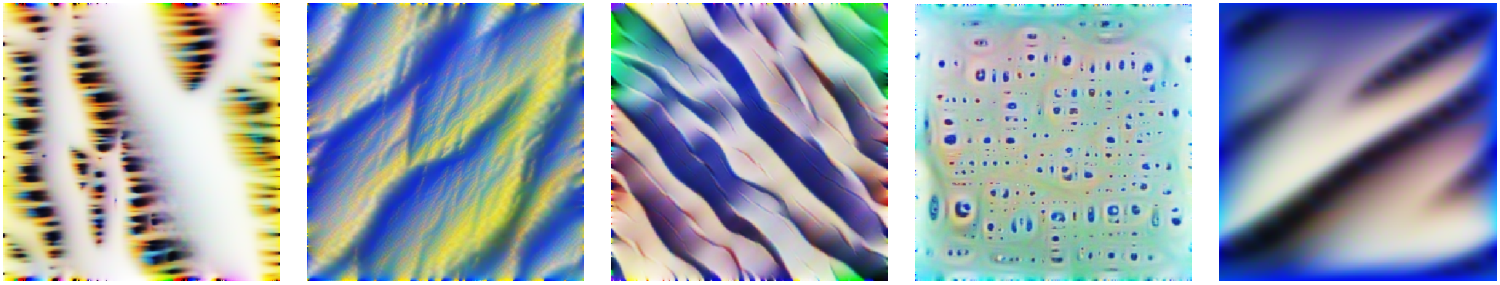
\includegraphics[width=0.98\linewidth]{figures/02_deep_learning/feature_vis/l11.pdf}
				} \\
				\subfloat[Layer $21$: patterns.]{
					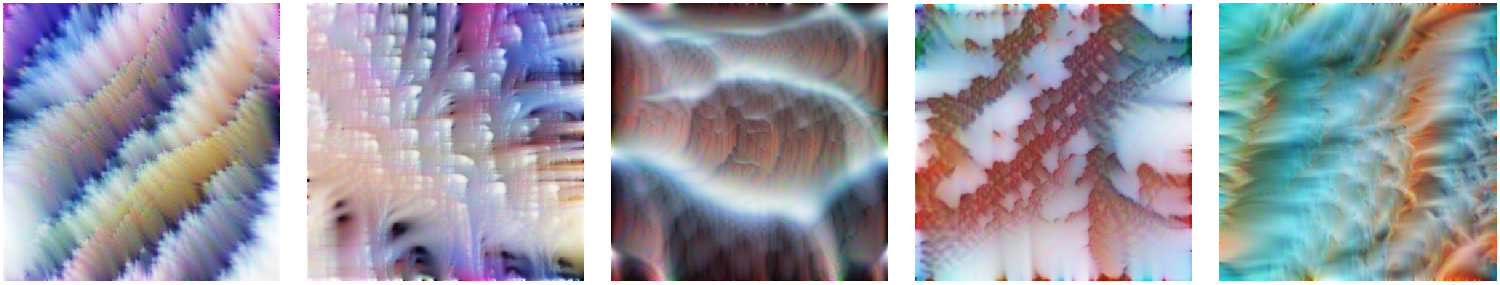
\includegraphics[width=0.98\linewidth]{figures/02_deep_learning/feature_vis/l21.pdf}
				} \\
				\subfloat[Layer $31$: parts.]{
					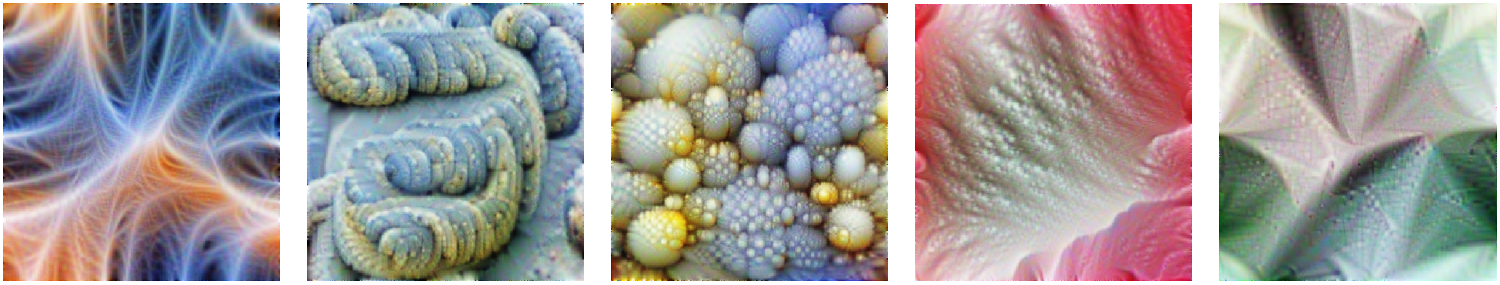
\includegraphics[width=0.98\linewidth]{figures/02_deep_learning/feature_vis/l31.pdf}
				} \\			
				\subfloat[Layer $41$: structures.]{
					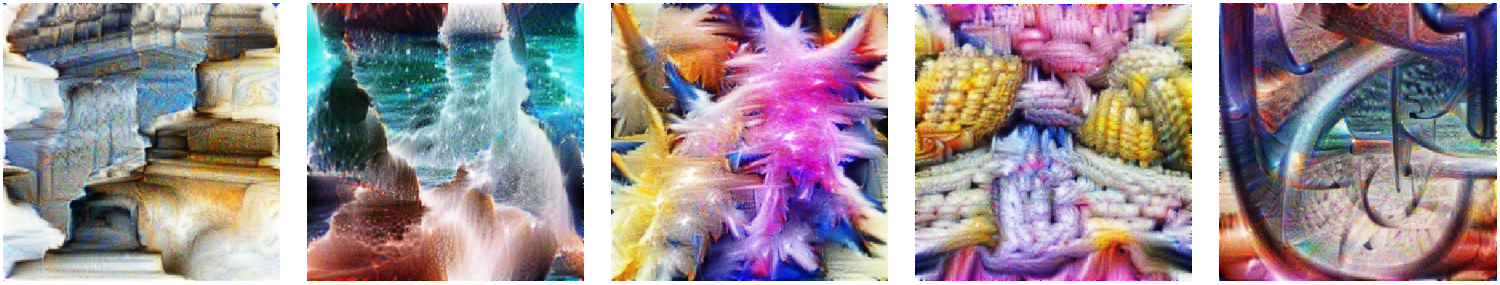
\includegraphics[width=0.98\linewidth]{figures/02_deep_learning/feature_vis/l41.pdf}
				}
				\caption[Feature visualizations from VGG16 layers]{Feature visualizations from VGG16 layers.}
				\label{fig:feature_vis_layers}
			\end{figure}
			
			\begin{figure}[!ht]
				\centering
				\subfloat[Scorpion]{
					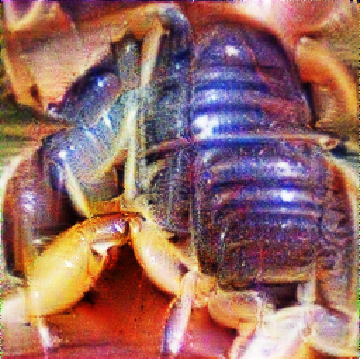
\includegraphics[width=0.30\linewidth]{figures/02_deep_learning/feature_vis/classes_01_scorpion.png}
				}
				\subfloat[Tarantula]{
					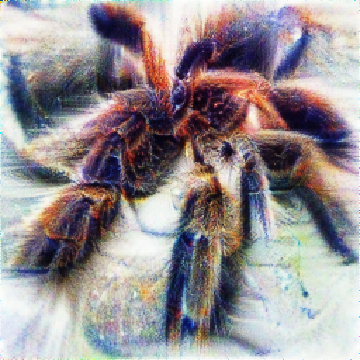
\includegraphics[width=0.30\linewidth]{figures/02_deep_learning/feature_vis/classes_02_tarantula.png}
				}
				\subfloat[Centipede]{
					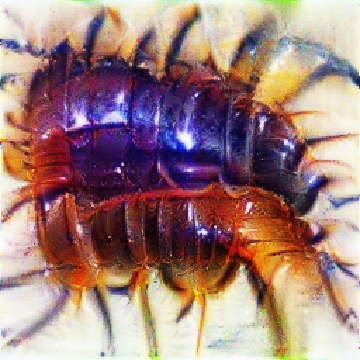
\includegraphics[width=0.30\linewidth]{figures/02_deep_learning/feature_vis/classes_03_centipede.png}
				} \\
				
				\subfloat[Seaslug]{
					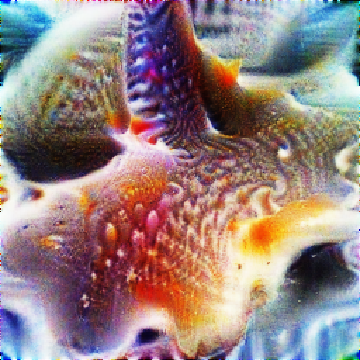
\includegraphics[width=0.30\linewidth]{figures/02_deep_learning/feature_vis/classes_11_seaslug.png}
				}
				\subfloat[Crab]{
					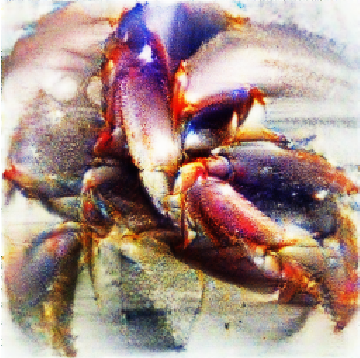
\includegraphics[width=0.30\linewidth]{figures/02_deep_learning/feature_vis/classes_12_crab.png}
				}
				\subfloat[Stork]{
					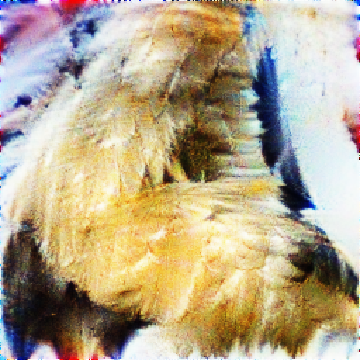
\includegraphics[width=0.30\linewidth]{figures/02_deep_learning/feature_vis/classes_13_stork.png}
				} \\
				
				\subfloat[Unicycle]{
					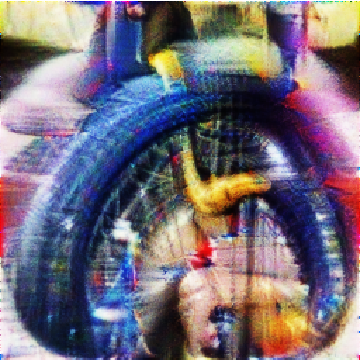
\includegraphics[width=0.30\linewidth]{figures/02_deep_learning/feature_vis/classes_21_unicycle.png}
				}
				\subfloat[Violin]{
					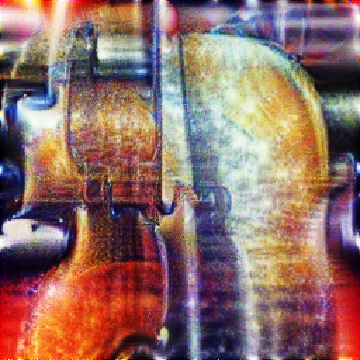
\includegraphics[width=0.30\linewidth]{figures/02_deep_learning/feature_vis/classes_22_violin.png}
				}
				\subfloat[Wallclock]{
					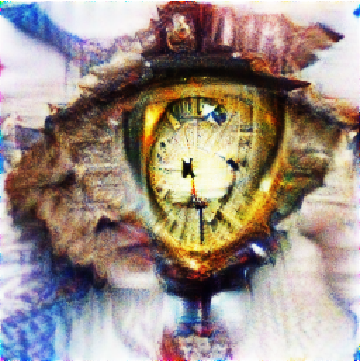
\includegraphics[width=0.30\linewidth]{figures/02_deep_learning/feature_vis/classes_23_wallclock.png}
				}	
				\caption[Class visualizations from VGG16]{Visualization of classes learned by VGG16.}
				\label{fig:feature_vis_classes}
			\end{figure}
	
	\section{Deep Learning in Mobile Networks}
	
		% Rolf Stadler papers
		
		% Online feature selection
		% https://ieeexplore.ieee.org/abstract/document/9269066
		% https://arxiv.org/pdf/2112.08253.pdf
		
		% Service metrics
		% - Prediction distributions - https://ieeexplore.ieee.org/abstract/document/8584941
		% - Efficient learning on high dimensional data - https://ieeexplore.ieee.org/abstract/document/9012741
		% - Conditional density estimation - https://ieeexplore.ieee.org/abstract/document/9422765
		
		% Security strategies through reinforcement learning
		% https://ieeexplore.ieee.org/abstract/document/9269092
		
		% Online learning under resource constraints
		% https://ieeexplore.ieee.org/abstract/document/9464066
	
		\subsection{State-of-the-art}
			\label{cha:deep_learning:sec:related_work}
			
			Using the so far collected understanding of how deep learning and deep neural nets work and how they should be used, we can now take a critical look at how deep learning is utilized in mobile networks.
			\ac{5G} is the first mobile network generation that is meant to depend on advanced \ac{ML} techniques.
			In \ac{5G},	deep learning is regarded as both the solution to overcome the exponentially increasing complexity, and the enabler for many of the use cases previously thought to be impossible.
			\ac{5G} is already under development for some years now, so naturally, quite a volume of literature is available on deep learning in \ac{5G} networks.
			The different areas where \ac{DL} could be utilized are well summarized \cite{dl_mobile_survey}, also depicted in Fig.~\ref{fig:dl_mobile_uses}, and advanced use cases are detailed in \cite{can_book}.
			Some areas fall outside the boundaries of network automation: these are either low-level, real-time tasks (such as signal processing), or application-level tasks (such as application-level data analysis, or deep-learning-based applications).
			
			\begin{figure}[ht]
				\centering
				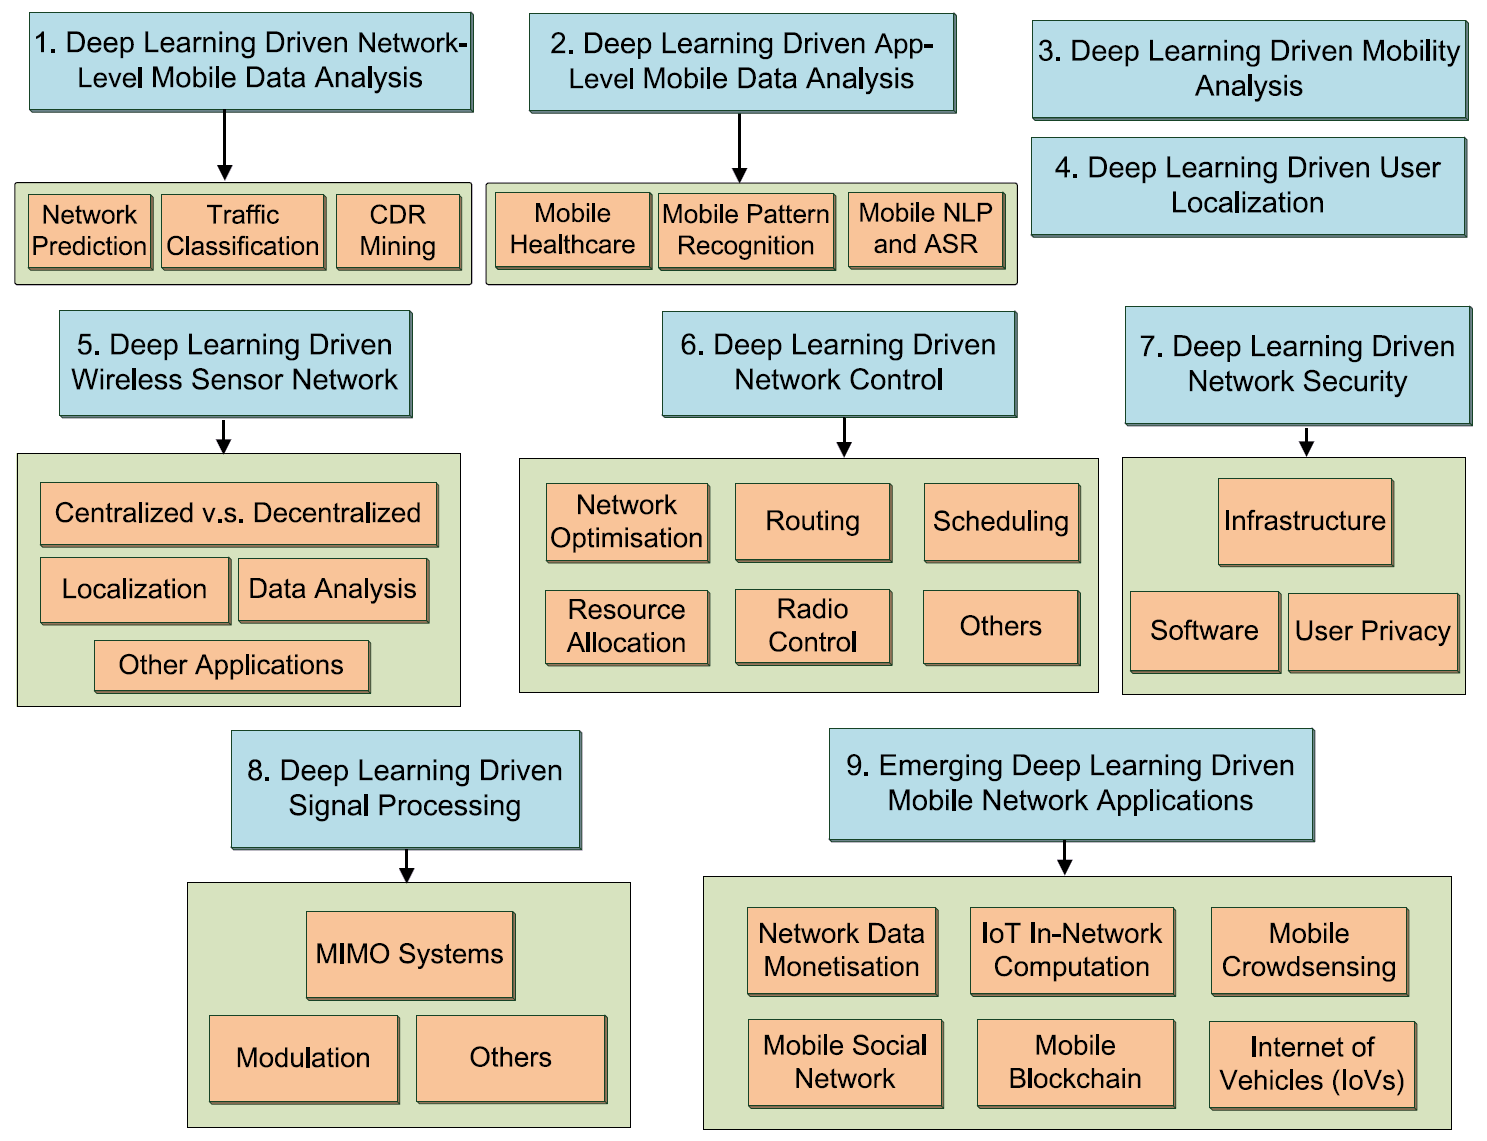
\includegraphics[width=\linewidth]{figures/02_deep_learning/dl_mobile_uses/dl_mobile_uses.png}
				\caption[DL topics in network automation]{Overview of topics in network automation utilizing deep learning \cite{dl_mobile_survey}.}
				\label{fig:dl_mobile_uses}
			\end{figure}
			
			The categories that fit the scope of (cognitive) network automation are:			
			\begin{itemize}
				\item \textbf{Learning Driven Network-Level Mobile Data Analysis:}
				Use cases here include traffic classification or \ac{QoE} from related, easily measurable \ac{QoS} \acp{KPI}.
				Another example is cell anomaly detection; detection of hardware or software faults, or misconfigurations using \acp{KPI} describing per-cell behavior.
				Yet another use case in this category is the long-term prediction of traffic or user growth, aiding network planning by predicting long-term demand.
				
				\item \textbf{Deep Learning Driven User Localization:}
				These use case cover the precise estimation of the user position using various localization techniques, to support location-based functionality, such as \ac{MDT} or mobility analysis.
				
				\item \textbf{Deep Learning Driven Mobility Analysis:}
				These use cases use the prediction of individual, or large crowd movement through wireless networks, for load balancing or predictive handover triggers in availability-critical services, such as \ac{URLLC}.
				
				\item \textbf{Deep Learning Driven Network Control:}
				Use cases here include dynamic resource allocation tasks, such as \ac{RRC}, routing or scheduling.
				An example of a resource allocation task is predictive network slicing, allocating multiple types of resources to services or users in the network.
				
				\item \textbf{Deep Learning Driven Network Security:}
				Use cases such as the detection of traffic anomalies, which can signal man-in-the-middle attacks, botnets or other security risks in the network.
			\end{itemize}		
			\noindent These categories all could utilize \ac{DL} in order to make decisions or to extract insight from a large variety and volume of data.
			However, not all of these possible \ac{DL} landing zones are actually considered, or do not utilize \ac{DL} to its fullest capabilities, as we will see shortly.
			
			% ------------------------------------------------------------------------------------------------------------------------------------------------------------------
			% Surveys + Summaries
			% ------------------------------------------------------------------------------------------------------------------------------------------------------------------
			
			% * AI for 5G: research directions and paradigms
			% * Intelligent 5G: When Cellular Networks Meet Artificial Intelligence
			% * Artificial Intelligence in 5G Technology: A Survey		
			
			% * Deep learning at the physical layer: System challenges and applications to 5G and beyond
			% * Deep learning for physical-layer 5G wireless techniques: Opportunities, challenges and solutions
			
			Different \ac{ML} techniques are often (incorrectly) referred to under the umbrella term \ac{AI} in mobile networks literature.
			The list of \ac{ML} algorithms that span the \ac{AI} ``spectrum'' is quite wide: complexity can range from simple statistical algorithms, such as linear regression, all the way to deep reinforcement learning algorithms using \acp{DQN}.
			This ``overselling'' is a constant problem in mobile network literature, which makes it hard to judge the actual capabilities of the utilized \ac{ML} algorithms at first glance, especially in surveys exploring the use of \ac{AI} in mobile networks.
			Most surveys recognize at least the $3$ main \ac{ML} principles, and refer to the following \ac{ML} algorithms in each principle \cite{ai_for_5g, ai_in_5g, intelligent_5g}:
			\begin{enumerate}[label=\textbf{\alph*})]
				\item \textbf{Supervised learning:}
				Supervised learning is the most commonly discussed \ac{ML} principle in surveys, and also contains the most complex learning algorithms.
				\ac{ML} algorithms that are utilized here include \ac{LR}, \acp{SVM}, \acp{HMM}, decision trees, and neural nets (the depth of which will be discussed shortly).
				Supervised learning is thought to be useful in tasks in all levels of the network, from root-cause analysis in network management all the way to channel estimation close to the physical layer.		
				This category usually also includes prediction tasks, which I don't consider as supervised-learning-based on the lack of human input needed for training data preparation (Sec.~\ref{cha:intro:sec:cognitive_cap_dl}).
				
				\item \textbf{Unsupervised learning:}
				Unsupervised learning is the least discussed principle in literature.
				The algorithms utilized here are often quite simple statistical methods, such as \ac{PCA}, \kmeans{}, \acp{GMM}, hierarchical and spectral clustering.
				More complex, but not deep learning capable algorithms include single class \acp{SVM} and \acp{SOM}.
				Deep learning capable neural nets, such as \acp{LSTM} are only discussed in the context of prediction, with the caveat of a strongly restricted model complexity because of the need for a short inference time in low-level tasks.
				Typically, unsupervised learning in higher-level (management) tasks are considered only to support the generation of labeled training datasets for later supervised learning algorithms, which actually implement the management functionality \cite{ai_for_5g}.
				
				\item \textbf{Reinforcement learning:}
				Reinforcement learning is an often discussed tool in the context of optimization tasks, such as resource allocation or self-configuration, or even in high-level management or network planning tasks.
				The reinforcement learning principle by nature requires quite complex algorithms, which range from the more traditional Q-learning to recent \acp{DQN}, often utilizing deep neural nets such as \acp{LSTM}.
			\end{enumerate}	
		
			% Individual papers		
			% ------------------------------------------------------------------------------------------------------------------------------------------------------------------
			% Organizing per topic
			% ------------------------------------------------------------------------------------------------------------------------------------------------------------------
			
			% Short-timeframe radio interface control
			% * Deep learning-based mmWave beam selection for 5G NR/6G with sub-6 GHz channel information: Algorithms and prototype validation - Beam selection  - Supervised Classification (Deep FC net)
			% * Deep learning based pilot allocation scheme (DL-PAS) for 5G massive MIMO system - Short timeframe MIMO/Beam control - Supervised Classification (Shallow FC) 
			% * A deep-learning-based radio resource assignment technique for 5G ultra dense networks - Short timeframe RRC - ? Prediction (Shallow LSTM)
			% * Deep learning for radio resource allocation with diverse quality-of-service requirements in 5g - Short timeframe RRC - Supervised Regression (Two Shallow FC nets)
			% * Channel state information prediction for 5G wireless communications: A deep learning approach - Channel quality prediction - Short-timeframe Sequence Prediction (Quite deep CNN + LSTM)
			% * Performance Evaluation of Channel Decoding with Deep Neural Networks - Channel decoding - Supervised regression (shallow MLP, CNN and RNN, authors say restrictive)
			
			% High-level resource allocation
			% * Deep reinforcement learning for dynamic computation offloading and resource allocation in cache-assisted mobile edge computing systems - MEC offloading and cache allocation w/ reinforcement learning - DQN
			% * Intelligent Offloading in Multi-Access Edge Computing: A State-of-the-Art Review and Framework - Placement in MEC - DQN
			% * A deep reinforcement learning based framework for power-efficient resource allocation in cloud RANs - Cloud RAN resource allocation - DQN
			% 
			% * DeepCog: Cognitive network management in sliced 5G networks with deep learning - Slicing - Supervised Prediction (Medium Deep 3D CNN + FC)
			% * Deep Reinforcement Learning for Resource Management in Network Slicing - Network Slicing resource allocation - DQN		
			% * Deepslice: A deep learning approach towards an efficient and reliable network slicing in 5G networks - Network slice prediction - Fancy Classification (which slice it should be assigned) (Shallow FC net)
			
			% Traffic anomaly detection
			% * A self-adaptive deep learning-based system for anomaly detection in 5G networks - Traffic anomaly detection (security) - Supervised Classification (Shallow FC (DBN, SAE)) 
			% * An efficient deep learning model for intrusion classification and prediction in 5G and IoT networks - Traffic anomaly detection (security)  - AE pretraining + Supervised Classification (AE ?, classifier shallow FC net)
			% * Deep Learning-Based Big Data-Assisted Anomaly Detection in Cellular Networks - Sleeping cells finally - Supervised classification (Quite deep MLP)
			
			% Outlier:
			% * Deep learning for hybrid 5G services in mobile edge computing systems: Learn from a digital twin - User association w/ digital twin (mobility, association, offloading) - Prediction (lables w/ twin) (Shallow-medium FC net)
			
			The above referenced surveys discuss a quite broad range of algorithms with varying complexity, and in my opinion provide an unfocused view of what constitutes today as deep learning in mobile networks.
			In order to get a representative, unbiased view of what is currently discussed as deep learning in \ac{5G}, I conducted my own survey by searching for papers which include the ``\ac{5G}'' and ``deep learning'' keywords on IEEEXplore\footnote{\url{https://ieeexplore.ieee.org/}}.
			The below papers were gathered by sorting the results from the query by the decreasing number of citations.
			I manually selected papers which are a) on the topic of mobile network operation on all levels (but not applications in mobile networks which use \ac{DL}) and b) reasonably recent.
			I found that most of the papers can be organized into $3$ use case groups:
			\begin{enumerate}[label=\textbf{\alph*})]
				\item 
					\textbf{Short-timeframe radio interface control:}
					These tasks involve the reconfiguration of the radio interface such as \ac{MIMO} control or beam selection \cite{dl_based_beam_select, dl_based_pilot_alloc}, \ac{RRC} \cite{dl_based_rrc, dl_for_rrc}, the prediction of channel quality \cite{channel_state_pred} or even the task of channel decoding itself \cite{channel_decoding_dl}.
					These tasks require frequent inference cycles, often close to per \ac{TTI} ($10$s of milliseconds), while in even more extreme cases, such as channel decoding, latency budgets for inference are as small as only a few microseconds \cite{dl_phys_survey}.
					A further constraint is the limited computational capacity available in mobile devices, as well as the need to conserve battery life with lightweight algorithms.
					All these constraints limit the allowed complexity of the \ac{DL} algorithms used close to the physical layer, which for neural nets means the limitation of layer widths and the number of layers in order to reduce the number of weights/parameters in the net \cite{dl_phys_survey2}.
					Most of them use shallow \ac{FC} or convolutional nets, or simple \acp{LSTM}, which limits the ``deep'' learning capacity of these nets by reducing the number of hierarchical features to be possibly learned.
					The majority of these works use some form of supervised learning, such as classification, or regression to a predefined function found by convex optimization or exhaustive search.
				
				\item
					\textbf{High-level resource allocation:}
					A large portion of these works involve the resource allocation in cloud environments, such as intelligently caching or offloading applications in \ac{MEC} \cite{mec_offload_cache, mec_offload}, or resource allocation in cloud-\ac{RAN} \cite{cloud_ran_resource}.
					These tasks are frequently solved with reinforcement learning, often utilizing \acp{DQN} to learn and optimize a resource allocation strategy in a simulated environment.
					Other, even more complex vertical resource allocation tasks involve network slicing, where both physical and virtual resources are allocated end-to-end in the network for user types or applications \cite{slicing_resource, drl_slicing_resource, slicing_resource2}.
					Network slicing papers often use classification as an \ac{ML} principle, as well as reinforcement learning, in both of which the nets used can be quite deep and thus realize deep learning.
							
				\item
					\textbf{Traffic anomaly detection:}
					This area is involved in the detection of anomalous traffic patterns in the network, which could stem from malicious attacks such as botnets \cite{anomaly_botnet}, intrusions over radio \cite{anomaly_intrusion}, or software or hardware failures \cite{anomaly_sleeping}.
					Although anomaly detection could be undertaken with unsupervised algorithms, by modeling normal behavior and detecting patterns that fall outside of this model, most of the current works use supervised learning algorithms.
					With supervised learning and the correct dataset, generally, a higher precision can be achieved with much simpler models, which is also represented in the quite shallow \ac{FC} nets used by these works.
					Unfortunately, this also limits the capability of these nets to learn hierarchical features, thus not really realizing deep learning.		
			\end{enumerate}
		
			Many of the listed works utilize shallow, simple neural nets, which would not be necessarily considered as deep-learning-capable.
			This is especially true in low-level tasks close to the physical layer, where inference execution time is limited.
			High-level, large-scale or management-oriented tasks don't suffer from these timing constraints, thus the possibility to employ \ac{DL} is greater here.
			However, often in these tasks the amount of data needed to truly utilize the capabilities of \ac{DL} is overwhelming, and is not yet supported or produced by current mobile networks, thus researchers tend to fall back to simpler \ac{ML} models.
			Workarounds to this problem exist, such as the utilization of complex digital twins to produce training data for these high-level tasks \cite{dl_digital_twin}, but this usually requires extraordinary effort for many tasks and is simply not available for most researchers.			
			
			My takeaway is that deep learning is too often used only as a buzzword in \ac{5G}-related papers: while I don't doubt the possible benefits of using \ac{DL} for the above tasks, I question whether the employed \ac{ML} algorithms are truly capable of deep learning.
			Furthermore, in places where complex unsupervised \ac{DL} algorithms could provide the benefit of robustness or adaptability, instead simpler, supervised algorithms are used to achieve a small accuracy gain of a few percentage points.
			I think investigating unsupervised deep learning in many of these tasks could be worthwhile and provide a benefit over current solutions, or allow for new use cases.			

		\subsection{Drivers, Enablers and Constraints of DL}
			\label{cha:deep_learning:sec:constraints}
			
			The capability of deep neural nets comes at cost: with great cognitive power come great computational requirements.
			For deep neural nets, the drivers and constraints are intertwined, creating a complex landscape through which one must navigate when aiming to develop these algorithms.
			
			\subsubsection*{Computational power}
			
				As the basic steps to train neural nets through backpropagation and gradient descent are very atomic algebraic tasks, there is little room to algorithmically optimize these calculations.
				However, as these tasks are highly parallelizable, there are significant opportunities to speed up the computation through implementations using hardware capable of massively parallel computations.
				This has created a two-step cycle of progression for \acp{DNN}:
				\begin{enumerate}[label=\textbf{\alph*})]
					\item Neural nets are improved, allowing for deeper, more complex topologies to be trained but with major increases in computational requirements.
					\item Hardware capabilities and storage capacity is improved, allowing for the complex \acp{DNN} to be trained and tested in humanly acceptable timeframes, e.g., purpose-built hardware and new implementations emerge to further speed up computations.				
				\end{enumerate}
				\noindent Nowadays, all but the simplest neural nets require dedicated hardware -- usually in the form of \acp{GPU} -- to train and infer within a reasonable time.
				These \acp{GPU} are slowly becoming more and more widespread both in end-user devices (mobile phones), and in the network itself (edge clouds).
				However, running the inference on either side is problematic: mobile phones have a limited battery life, and should conserve it by minimizing \ac{DL} computation.
				This can be achieved by offloading computation to the edge cloud, but in this, case the amount of data communicated can be overwhelming, or security and privacy concerns can emerge if the user's data is sensitive.
			
			\subsubsection*{Timing constraints}
			
				Current improvements sometimes achieve only a few $1/10$ of a percent increase in accuracy at the cost of a $10$-fold increase in training and inference time.
				However, these seemingly small increments in accuracy amount to a large forward-step in cognitional power need, which in turn means a significant increase in processing time.
				Deep neural nets can have two types of constraints for processing time:
				\begin{enumerate}[label=\textbf{\alph*})]
					\item A hard time-limit at inference, so that the net is able to process the constant stream of information at the rate it is arriving, such as the case with object recognition in video processing.
					\item A softer time-limit at training, so that the neural net can be trained in a reasonable timeframe.
				\end{enumerate}	
				\noindent The time it takes to develop a concept into prototype -- mainly influenced by the models’ training time -- is critical in deep learning research.
				Although most common architectures nowadays can be trained on desktop computers, the need for speed and simplicity implies that buying expensive, specialized hardware dedicated to deep learning is not a waste.
				This is the reason why the leading institutions in the field utilize huge supercomputers; being able to validate a concept quickly without spending much effort on optimization is invaluable in the deep learning race.
			
			\subsubsection*{Quantity of data}
			
				The companies most invested in deep learning are those that handle large amounts of data, usually in the form of images, videos, or text, where the automation of tasks previously solved by humans would mean a huge decrease in cost and a large increase in capacity.
				This large amount of information, however, is not only a burden; the quantity and quality of available data is what enables the training of the learning machines more than any hardware or algorithmic improvement could.
				Within this lies a big problem for \ac{DL} in mobile networks: mobile network vendors -- the ones potentially developing the \ac{DL} algorithms -- are cut off from the source of the data, the large-scale mobile network deployments, as these are owned and run by network operators.
				Sharing data from network operators requires agreements on both sides, good cooperation and a lot of effort in order to maintain anonymity for the users, or avoid leaking sensitive information about the operator itself.
				This effort is seldom profitable for the operator, thus, they are usually reluctant to share data, leaving the vendors without access to the fundamental enabler of \ac{DL}.
					
			The consideration of these aspects of \ac{DL} is crucial when developing algorithms.
			Many good ideas on paper turn out to be problematic in one of the above topics, when a real deployment is considered in a mobile network.
			This is the reason why my research objectives include such considerations, and why these topics are going to be further discussed throughout this thesis.			
			
